\documentclass{article}
\author{Mike Hearn, Richard Gendal Brown}
\date{\today}
\title{Corda: A distributed ledger}
%%\setlength{\parskip}{\baselineskip}
\usepackage{amsfonts}
\usepackage{minted}
\usemintedstyle{vs}
\newminted{kotlin}{%
    breakbytoken,%
    breaklines,%
    autogobble,%
    frame=lines,%
    framesep=2\fboxsep,%
    fontsize=\footnotesize%
}
\usepackage{color}
\usepackage{epigraph}
\usepackage{graphicx}
\graphicspath{ {images/} }
\usepackage[export]{adjustbox}
\usepackage{float}
\usepackage{hyperref}

% Get rid of ugly boxes around clickable links
\usepackage{xcolor}
\hypersetup{
    colorlinks,
    linkcolor={blue!50!black},
    citecolor={blue!50!black},
    urlcolor={blue!80!black}
}

\usepackage[super,comma,sort&compress]{natbib}
\usepackage[nottoc]{tocbibind}
\usepackage[parfill]{parskip}
\usepackage{textcomp}
\usepackage{scrextend}
\usepackage{cleveref}
\usepackage{csquotes}
\crefformat{section}{\S#2#1#3}
\addtokomafont{labelinglabel}{\sffamily}
%\usepackage[natbibapa]{apacite}
\renewcommand{\thefootnote}{\alph{footnote}}
%\epigraphfontsize{\small\itshape}
\setlength\epigraphwidth{4.5cm}
\setlength\epigraphrule{0pt}

\begin{document}

\maketitle
\begin{center}
Version 1.0
\end{center}

\vspace{10mm}

\begin{abstract}

A decentralised database with minimal trust between nodes would allow for the creation of a global ledger. Such a ledger
would have many useful applications in finance, trade, healthcare and more. We present Corda, a decentralised
global database, and describe in detail how it achieves the goal of providing a platform for decentralised app
development. We elaborate on the high level description provided in the paper \emph{Corda: An
introduction}\cite{CordaIntro} and provide a detailed technical discussion.

\end{abstract}
\vfill

\newpage
\tableofcontents
\newpage
\section{Introduction}

In many industries significant effort is needed to keep organisation specific databases in sync with each other. In
the financial sector the effort of keeping different databases synchronised, reconciling them to ensure they
actually are synchronised and resolving the `breaks' that occur when they are not represents a significant fraction
of the total work a bank actually does.

Why not just use a shared relational database? This would certainly solve a lot of problems using only existing
technology, but it would also raise more questions than answers:

\begin{itemize}
\item Who would run this database? Where would we find a sufficient supply of angels to own it?
\item In which countries would it be hosted? What would stop that country abusing the mountain of sensitive information it would have?
\item What if it were hacked?
\item Can you actually scale a relational database to fit the entire financial system?
\item What happens if the database needs to go down for maintenance? Does the economy stop?
\item What kind of nightmarish IT bureaucracy would guard schema changes?
\item How would you manage access control?
\end{itemize}

We can imagine many other questions. A decentralised database attempts to answer them.

In this paper we differentiate between a \emph{decentralised} database and a \emph{distributed} database. A
distributed database like BigTable\cite{BigTable} scales to large datasets and transaction volumes by spreading the
data over many computers. However it is assumed that the computers in question are all run by a single homogeneous
organisation and that the nodes comprising the database all trust each other not to misbehave or leak data. In a
decentralised database, such as the one underpinning Bitcoin\cite{Bitcoin}, the nodes make much weaker trust
assumptions and actively cross-check each other's work. Such databases trade performance and usability for security
and global acceptance.

\emph{Corda} is a decentralised database platform with the following novel features:

\begin{itemize}
\item Nodes are arranged in an authenticated peer to peer network. All communication is direct. Gossip is not used.
\item New transaction types can be defined using JVM\cite{JVM} bytecode. The bytecode is statically analyzed and rewritten
on the fly to be fully deterministic, and to implement deterministic execution time quotas.
\item Transactions may execute in parallel, on different nodes, without either node being aware of the other's transactions.
\item There is no block chain\cite{Bitcoin}. Transaction races are deconflicted using pluggable \emph{notaries}. A single
Corda network may contain multiple notaries that provide their guarantees using a variety of different algorithms. Thus
Corda is not tied to any particular consensus algorithm. (\cref{sec:notaries})
\item Data is shared on a need-to-know basis. Nodes provide the dependency graph of a transaction they are sending to
another node on demand, but there is no global broadcast of \emph{all} transactions.
\item Bytecode-to-bytecode transformation is used to allow complex, multi-step transaction building protocols called
\emph{flows} to be modelled as blocking code. The code is transformed into an asynchronous state machine, with
checkpoints written to the node's backing database when messages are sent and received. A node may potentially have
millions of flows active at once and they may last days, across node restarts and even certain kinds of upgrade. Flows expose progress
information to node administrators and users and may interact with people as well as other nodes. A library of flows is provided
to enable developers to re-use common protocols such as notarisation, membership broadcast and so on.
\item The data model allows for arbitrary object graphs to be stored in the ledger. These graphs are called \emph{states} and are the atomic unit of data.
\item Nodes are backed by a relational database and data placed in the ledger can be queried using SQL as well as joined
with private tables. States can declare a relational mapping using the Java Persistence Architecture standard (JPA)~\cite{JPA}.
\item The platform provides a rich type system for the representation of things like dates, currencies, legal entities and
financial entities such as cash, issuance, deals and so on.
\item The network can support rapid bulk data imports from other database systems without placing load on the network.
Events on the ledger are exposed via an embedded JMS compatible message broker.
\item States can declare scheduled events. For example a bond state may declare an automatic transition to an
``in default'' state if it is not repaid in time.
\item Advanced privacy controls allow users to anonymize identities, and initial support is provided for running
smart contracts inside memory spaces encrypted and protected by Intel SGX.
\end{itemize}

Corda follows a general philosophy of reusing existing proven software systems and infrastructure where possible.
Comparisons with Bitcoin and Ethereum will be provided throughout.

\newpage

\section{Overview}

Corda is a platform for the writing and execution of ``CorDapps'': applications that extend the global database
with new capabilities. Such apps define new data types, new inter-node protocol flows and the so-called ``smart
contracts'' that determine allowed changes.

What is a smart contract? That depends on the model of computation we are talking about. There are two competing
computational models used in decentralised databases: the virtual computer model and the UTXO model. The virtual
computer model is used by Ethereum\cite{Ethereum} and Hyperledger Fabric. It models the database as the in-memory
state of a global computer with a single thread of execution determined by the block chain. In the UTXO model, as
used in Bitcoin, the database is a set of immutable rows keyed by \texttt{(hash:output index)}. Transactions define
outputs that append new rows and inputs which consume existing rows. The term ``smart contract'' has a different
meaning in each model. A deeper discussion of the tradeoffs and terminology in the different approaches can be
found in the Corda introductory paper\cite{CordaIntro}.

We use the UTXO model and as a result our transactions are structurally similar to Bitcoin transactions: they have
inputs, outputs and signatures. Unlike Bitcoin, Corda database rows can contain arbitrary data, not just a value
field. Because the data consumed and added by transactions is not necessarily a set of key/value pairs, we don't
talk about rows but rather \emph{states}. Like Bitcoin, Corda states are associated with bytecode programs that
must accept a transaction for it to be valid, but unlike Bitcoin, a transaction must satisfy the programs for both
the input and output states at once. \emph{Issuance transactions} may append new states to the database without
consuming any existing states but unlike in Bitcoin these transactions are not special and may be created at any
time, by anyone.

In contrast to both Bitcoin and Ethereum, Corda does not order transactions using a block chain and by implication
does not use miners or proof-of-work. Instead each state points to a \emph{notary}, which is a service that
guarantees it will sign a transaction only if all the input states are un-consumed. A transaction is not allowed to
consume states controlled by multiple notaries and thus there is never any need for two-phase commit between
notaries. If a combination of states would cross notaries then a special transaction type is used to move them onto
a single notary first. See~\cref{sec:notaries} for more information.

The Corda transaction format has various other features which are described in later sections.

\section{The peer to peer network}

\subsection{Overview}

A Corda network consists of the following components:

\begin{itemize}
\item Nodes, operated by \emph{parties}, communicating using AMQP/1.0 over TLS.
\item An \emph{identity} service which runs an X.509 certificate authority.
\item A network map service that publishes information about how to connect to nodes on the network.
\item One or more notary services. A notary may be decentralised over a coalition of different parties.
\item Zero or more oracle services. An oracle is a well known service that signs transactions if they state a fact
and that fact is considered to be true. They may also optionally also provide the facts. This is how the ledger can be
connected to the real world, despite being fully deterministic.
\end{itemize}

% TODO: Add section on zones and network parameters

Oracles and notaries are covered in later sections.

\subsection{The identity root}\label{subsec:the-identity-root}

Taking part in a Corda network as a node requires an identity certificate. These certificates bind a human readable
name to a public key and are signed by the network operator. Having a signed identity grants the ability to take
part in the top layer of the network, but it's important to understand that users can participate in the ledger
\emph{without} having an issued identity. Only a raw key pair is necessary if a node that \emph{does} have an
identity is willing to route traffic on your behalf. This structure is similar to the email network, in which users
without servers can take part by convincing a server operator to grant them an account. How network identities and
accounts relate to each other is discussed in a later section (section~\cref{sec:identity}).

This `identity' does not have to be a legal or true name. In the same way that an email address is a globally
unique pseudonym that is ultimately rooted by the top of the DNS hierarchy, so too can a Corda network use
arbitrary self-selected usernames. The permissioning service can implement any policy it likes as long as the
identities it signs are globally unique. Thus it's possible to build an entirely pseudonymous Corda network.

However, when a network has a way to map identities to some sort of real world thing that's difficult to bulk create
many efficient and useful algorithms become available. Most importantly, all efficient byzantine fault tolerant
consensus algorithms require nodes to be usefully distinct such that users can reason about the likelihood of cluster
members going bad simultaneously. In the worst case where a BFT cluster consists of a single player pretending to be
several, the security of the system is completely voided in an undetectable manner. Useful privacy techniques like
mix networks and Tor\cite{Dingledine:2004:TSO:1251375.1251396} also make the assumption of unique, sybil-free
identities. For these reasons and more the mainline Corda network performs identity verification to require that
top-level members be companies, and it's recommended that all networks do so.

Identity is covered further in section~\cref{sec:identity}.

\subsection{The network map}

Every network requires a network map. This is similar to Tor's concept of \emph{directory authorities}. The network
map service publishes information about each node such as the set of IP addresses it listens on (multiple IP
addresses are supported for failover and load balancing purposes), the version of the protocol it speaks, and which
identity certificates it hosts. Each data structure describing a node is signed by the identity keys it claims to
host. The network map service is therefore not trusted to specify node data correctly, only to distribute it.

The network map abstracts the underlying network locations of the nodes to more useful business concepts like
identities and services. Domain names for the underlying IP addresses may be helpful for debugging but are not
required. User interfaces and APIs always work in terms of identities -- there is thus no equivalent to Bitcoin's
notion of an address (hashed public key), and user-facing applications rely on auto-completion and search rather
than QRcodes to identify a counterparty.

It is possible to subscribe to network map changes and registering with the map is the first thing a node does at
startup.

The map is a set of files that may be cached and distributed via HTTP based content delivery networks. The
underlying map infrastructure is therefore not required to be highly available: if the map service becomes
unreachable nodes may not join the network or change IP addresses, but otherwise things continue as normal.

\subsection{Message delivery}

The network is structurally similar to the email network. Nodes are expected to be long lived but may depart
temporarily due to crashes, connectivity interruptions or maintenance. Messages are written to disk and delivery is
retried until the remote node has acknowledged a message, at which point it is expected to have either reliably
stored the message or processed it completely. Connections between nodes are built and torn down as needed: there
is no assumption of constant connectivity. An ideal network would be entirely flat with high quality connectivity
between all nodes, but Corda recognises that this is not always compatible with common network setups and thus the
message routing component of a node can be separated from the rest and run outside the firewall. Being outside the
firewall or in the firewall's `de-militarised zone' (DMZ) is required to ensure that nodes can connect to anyone on
the network, and be connected to in turn. In this way a node can be split into multiple sub-services that do not
have duplex connectivity yet can still take part in the network as first class citizens.

The reference implementation provides this functionality using the Apache Artemis message broker, through which it
obtains journalling, load balancing, flow control, high availability clustering, streaming of messages too large to
fit in RAM and many other useful features. The network uses the \emph{AMQP/1.0}\cite{AMQP} protocol which is a
widely implemented binary messaging standard, combined with TLS to secure messages in transit and authenticate the
endpoints.

\subsection{Serialization}\label{subsec:serialization}

All messages are encoded using an extended form of the AMQP/1.0 binary format (\emph{Advanced Message Queue
Protocol}\cite{AMQP}). Each message has a UUID set in an AMQP header which is used as a deduplication key, thus
accidentally redelivered messages will be ignored.

Messages may also have an associated organising 64-bit \emph{session ID}. Note that this is distinct from the AMQP
notion of a session. Sessions can be long lived and persist across node restarts and network outages. They exist in
order to group messages that are part of a \emph{flow}, described in more detail below.

Corda uses AMQP and extends it with more advanced types and embedded binary schemas, such that all messages are
self describing. Because ledger data typically represents business agreements and data, it may persist for years
and survive many upgrades and infrastructure changes. We require that data is always interpretable in strongly
typed form, even if that data has been stored to a context-free location like a file, or the clipboard.

Although based on AMQP, Corda's type system is fundamentally the Java type system. Java types are mapped to
AMQP/1.0 types whenever practical, but ledger data will frequently contain business types that the AMQP type system
does not define. Fortunately, AMQP is extensible and supports standard concepts like polymorphism and interfaces,
so it is straightforward to define a natural Java mapping. Type schemas are hashed to form a compact `fingerprint'
that identifies the type, which allows types to be connected to the embedded binary schemas that describe them and
which are useful for caching. The AMQP type system and schema language supports a form of annotations that we map
to Java annotations.

Object serialization frameworks must always consider security. Corda requires all types that may appear in
serialized streams to mark themselves as safe for deserialization, and objects are only created via their
constructors. Thus any data invariants that are enforced by constructors or setter methods are also enforced for
deserialized data. Additionally, requests to deserialize an object specify the expected types. These two mechanisms
block gadget-based attacks\cite{DeserialisingPickles}. Such attacks frequently affect any form of data
deserialization regardless of format, for example, they have been found not only in Java object serialization
frameworks but also JSON and XML parsers. They occur when a deserialization framework may instantiate too large a
space of types which were not written with malicious input in mind.

The serialization framework supports advanced forms of data evolution. When a stream is deserialized Corda attempts
to map it to the named Java classes. If those classes don't exactly match, a process called `evolution' is
triggered, which automatically maps the data as smoothly as possible. For example, deserializing an old object will
attempt to use a constructor that matches the serialized schema, allowing default values in new code to fill in the
gaps. When old code reads data from the future, new fields will be discarded if safe to do so. Various forms of
type adaptation are supported, and type-safe enums can have unknown values mapped to a default enum value as well.

If no suitable class is found at all, the framework performs \emph{class synthesis}. The embedded schema data will
be used to generate the bytecode for a suitable holder type and load it into the JVM on the fly. These new classes
will then be instantiated to hold the deserialized data. The new classes will implement any interfaces the schema
is specified as supporting if those interfaces are found on the Java classpath. In this way the framework supports
a form of generic programming. Tools can work with serialized data without having a copy of the app that generated
it. The returned objects can be accessed either using reflection, or a simple interface that automates accessing
properties by name and is just a friendlier way to access fields reflectively. Creating genuine object graphs like
this is superior to the typical approach of defining a format specific generic data holder type (XML's DOM
\texttt{Element}, \texttt{JSONObject} etc) because there is already a large ecosystem of tools and technologies
that know how to work with objects via reflection. Synthesised object graphs can be fed straight into JSON or YaML
serializers to get back text, inserted into a scripting engine for usage with dynamic languages like JavaScript or
Python, fed to JPA for database persistence and query or a Bean Validation engine for integrity checking, or even
used to automatically generate GUIs using a toolkit like MetaWidget\cite{MetaWidget} or
ReflectionUI\cite{ReflectionUI}.

\subsection{Network parameters}\label{subsec:network-parameters}

In any DLT system there are various tunable parameters whose correct values may not be known ahead of time, may
change, or may be things upon which reasonable people will always disagree. Corda extracts these into a notion of
\emph{network parameters}. Network parameters are encoded in a data structure, signed by the network operator and
distributed via the same infrastructure as the network map. All nodes in a network must follow the configuration
provided, otherwise consensus may not be achieved.

Some examples of network parameters are:

\begin{itemize}
    \item The list of notaries acceptable for use within the network.
    \item The largest acceptable peer to peer message in bytes.
    \item The largest acceptable transaction size in bytes.
    \item The event horizon (see below).
    \item The minimum platform version required to take part in the network.
\end{itemize}

This list is not exhaustive and new parameters are added from time to time.

The \emph{event horizon} is the span of time that is allowed to elapse before an offline node is considered to be
permanently gone. Once a peer has been offline for longer than the event horizon, any nodes that have been
communicating with it may kill any outstanding flows and erase knowledge of it from their databases. Typical values
for the event horizon are long, for example, 30 days. This gives nodes that are only intermittently connected
plenty of time to come online and resynchronise. Shorter values may lead to business processes being interrupted
due to transient infrastructure outages for which repairs are already in progress.

\paragraph{Flag days and hard forks.}There must be a mechanism for the parameters to be updated. Each signed
parameter structure contains an incrementing integer epoch. When a new set of parameters is being introduced, it
starts to be referenced by hash from the current network map and an activation date is supplied. Nodes download the
new parameters, validate them and then alert the administrator that the network is changing. For some parameters
the administrator is expected to manually review the change and accept it. Failure to do so before the activation
date (the ``flag day'') results in the node shutting down, as it would no longer be able to fulfil its purpose.
Network operators are expected to communicate and coordinate this process out of band; the protocol allows nodes to
publish what parameters they have accepted so acceptance can be monitored and the flag day can be changed if
so desired. Unlike in proof-of-work based block chain systems, there is no way to continue past an unacceptable
change in the network parameters and remain on the `losing side'. Thus the notion of flag days is subtly different
to the notion of a hard fork.

\subsection{Protocol versioning}\label{subsec:protocol-versioning}

The network protocol is versioned using a simple incrementing integer version number. There are no minor or patch
versions in the protocol definition itself: the versioning scheme is based on a commitment for the protocol
to always be backwards compatible. All nodes publish their current highest supported version in their signed
\texttt{NodeInfo} structure, so peers can always known ahead of time which protocol features are available to them
before creating or receiving connections.

The protocol data structures are reflected in the platform API, which is therefore versioned in an identical
manner. Apps may specify the minimum platform version they require, such that nodes will refuse to load apps that
would need newer features than are supported. The decision to unify the protocol and API versions implies that some
protocol versions may be effectively identical despite having different version numbers: this was deemed preferable
to requiring developers to understand and keep track of two similar-but-different versioning streams.

\paragraph{Mandatory upgrades.}The network operator may choose to require that nodes meet a minimum version number
via setting a network parameter.

This is useful because in DLT systems some types of new feature require everyone in a network to upgrade before
anyone can use it. This is usually because the feature affects how transactions should be validated, and thus any
node may encounter the new data during transaction verification even if no installed app uses it itself. In this
case the API will throw an exception if an attempt is made to use a new feature on a network where the minimum
version number is lower than the version in which the new feature was introduced. The network can then use a flag
day to increase the minimum platform version and thus activate the new features. Nodes that aren't new
enough to handle the network's minimum version shut down automatically unless overridden. Because mandatory
upgrades may be difficult to coordinate and enforce future versions of the platform may support outsourcing of
transaction verification to third party nodes or remote SGX enclaves.

Flag days mark the end of a process: it is the point by which the overwhelming majority of network participants are
expected to have upgraded to some minimum version, and whose date is expected to be set by the network operator to
achieve the right balance for their network between meeting the needs of those who wish to use features that
require that version, and those for whom upgrading is difficult. It should be noted that flag days are expected to
be relatively rare once Corda matures. In any case the majority of new features do not change the data model and so
don't require everybody on the network to upgrade before they can be used.

\paragraph{Target versioning.}The node supports `target versioning', in which the latest version the app was
tested against is advertised in its metadata. The node can use this to activate or deactivate workarounds for buggy
apps that may have accidentally baked in dependencies on undefined platform behaviours, or to enable the semantics
of an API to evolve without breaking backwards compatibility. For example, if an API returns a list of elements
that happened to be sorted in previous versions, but then ceases to be sorted due to performance optimisations,
this could potentially break apps that assumed a certain value would always be found at a certain index. Target
versioning can be used to keep apps working even as the platform underneath it evolves.

\section{Flow framework}\label{sec:flows}

\subsection{Overview}

It is common in decentralised ledger systems for complex multi-party protocols to be needed. The Bitcoin payment
channel protocol\cite{PaymentChannels} involves two parties putting money into a multi-signature pot, then
iterating with your counterparty a shared transaction that spends that pot, with extra transactions used for the
case where one party or the other fails to terminate properly. Such protocols typically involve reliable private
message passing, checkpointing to disk, signing of transactions, interaction with the p2p network, reporting
progress to the user, maintaining a complex state machine with timeouts and error cases, and possibly interacting
with internal systems on either side. All this can become quite involved. The implementation of payment channels in
the \texttt{bitcoinj} library is approximately 9000 lines of Java, very little of which involves cryptography.

As another example, the core Bitcoin protocol only allows you to append transactions to the ledger. Transmitting
other information that might be useful such as a text message, refund address, identity information and so on is
not supported and must be handled in some other way -- typically by wrapping the raw ledger transaction bytes in a
larger message that adds the desired metadata and giving responsibility for broadcasting the embedded transaction
to the recipient, as in Bitcoin's BIP 70\cite{BIP70}.

In Corda transaction data is not globally broadcast. Instead it is transmitted to the relevant parties only when
they need to see it. Moreover even quite simple use cases -- like sending cash -- may involve a multi-step
negotiation between counterparties and the involvement of a third party such as a notary. Additional information
that isn't put into the ledger is considered essential, as opposed to nice-to-have. Thus unlike traditional block
chain systems in which the primary form of communication is global broadcast, in Corda \emph{all} communication
takes the form of small multi-party sub-protocols called flows.

The flow framework presents a programming model that looks to the developer as if they have the ability to run
millions of long lived threads which can survive node restarts. APIs are provided to send and receive serialized
object graphs to and from other identities on the network, embed sub-flows, handle version evolution and report
progress to observers. In this way business logic can be expressed at a very high level, with the details of making
it reliable and efficient abstracted away. This is achieved with the following components.

\paragraph{Just-in-time state machine compiler.}Code that is written in a blocking manner typically cannot be
stopped and transparently restarted later. The first time a flow's \texttt{call} method is invoked a
bytecode-to-bytecode transformation occurs that rewrites the classes into a form that implements a resumable state
machine. These state machines are sometimes called coroutines, and the transformation engine Corda uses (Quasar) is
capable of rewriting code arbitrarily deep in the stack on the fly. The developer may thus break his or her logic
into multiple methods and classes, use loops, and generally structure their program as if it were executing in a
single blocking thread. There's only a small list of things they should not do: sleeping, accessing the
network outside of the framework, and blocking for long periods of time (upgrades require in-flight flows to finish).

\paragraph{Transparent checkpointing.}When a flow wishes to wait for a message from another party (or input from a
human being) the underlying stack frames are suspended onto the heap, then crawled and serialized into the node's
underlying relational database (however, the AMQP framework isn't used in this case). The written objects are
prefixed with small schema definitions that allow some measure of portability across changes to the layout of
objects, although portability across changes to the stack layout is left for future work. Flows are resumed and
suspended on demand, meaning it is feasible to have far more flows active at once than would fit in memory. The
checkpointing process is atomic with respect to changes to the database and acknowledgement of network messages.

\paragraph{Identity to IP address mapping.}Flows are written in terms of identities. The framework takes care of
routing messages to the right IP address for a given identity, following movements that may take place whilst the
flow is active and handling load balancing for multi-homed parties as appropriate.

\paragraph{A library of subflows.}Flows can invoke sub-flows, and a library of flows is provided to automate common
tasks like notarising a transaction or atomically swapping ownership of two assets.

\paragraph{Progress reporting.}Flows can provide a progress tracker that indicates which step they are up to. Steps
can have human-meaningful labels, along with other tagged data like a progress bar. Progress trackers are
hierarchical and steps can have sub-trackers for invoked sub-flows.

\paragraph{Flow hospital.}Flows can pause if they throw exceptions or explicitly request human assistance. A flow
that has stopped appears in the \emph{flow hospital} where the node's administrator may decide to kill the flow or
provide it with a solution. Some flows that end up in the hospital will be retried automatically by the node
itself, for example in case of database deadlocks that require a retry. Future versions of the framework may add
the ability to request manual solutions, which would be useful for cases where the other side isn't sure why
you are contacting them. For example, if the specified reason for sending a payment is not recognised, or
when the asset used for a payment is not considered acceptable.

For performance reasons messages sent over flows are protected only with TLS. This means messages sent via flows
are deniable unless explicitly signed by the application. Automatic signing and recording of flow contents may be
added in future.

Flows are identified using Java class names i.e. reverse DNS notation, and several are defined by the base
protocol. Note that the framework is not required to implement the wire protocols, it is just a development aid.

% TODO: Revisit this diagram once it matches the text more closely.
%\begin{figure}[H]
%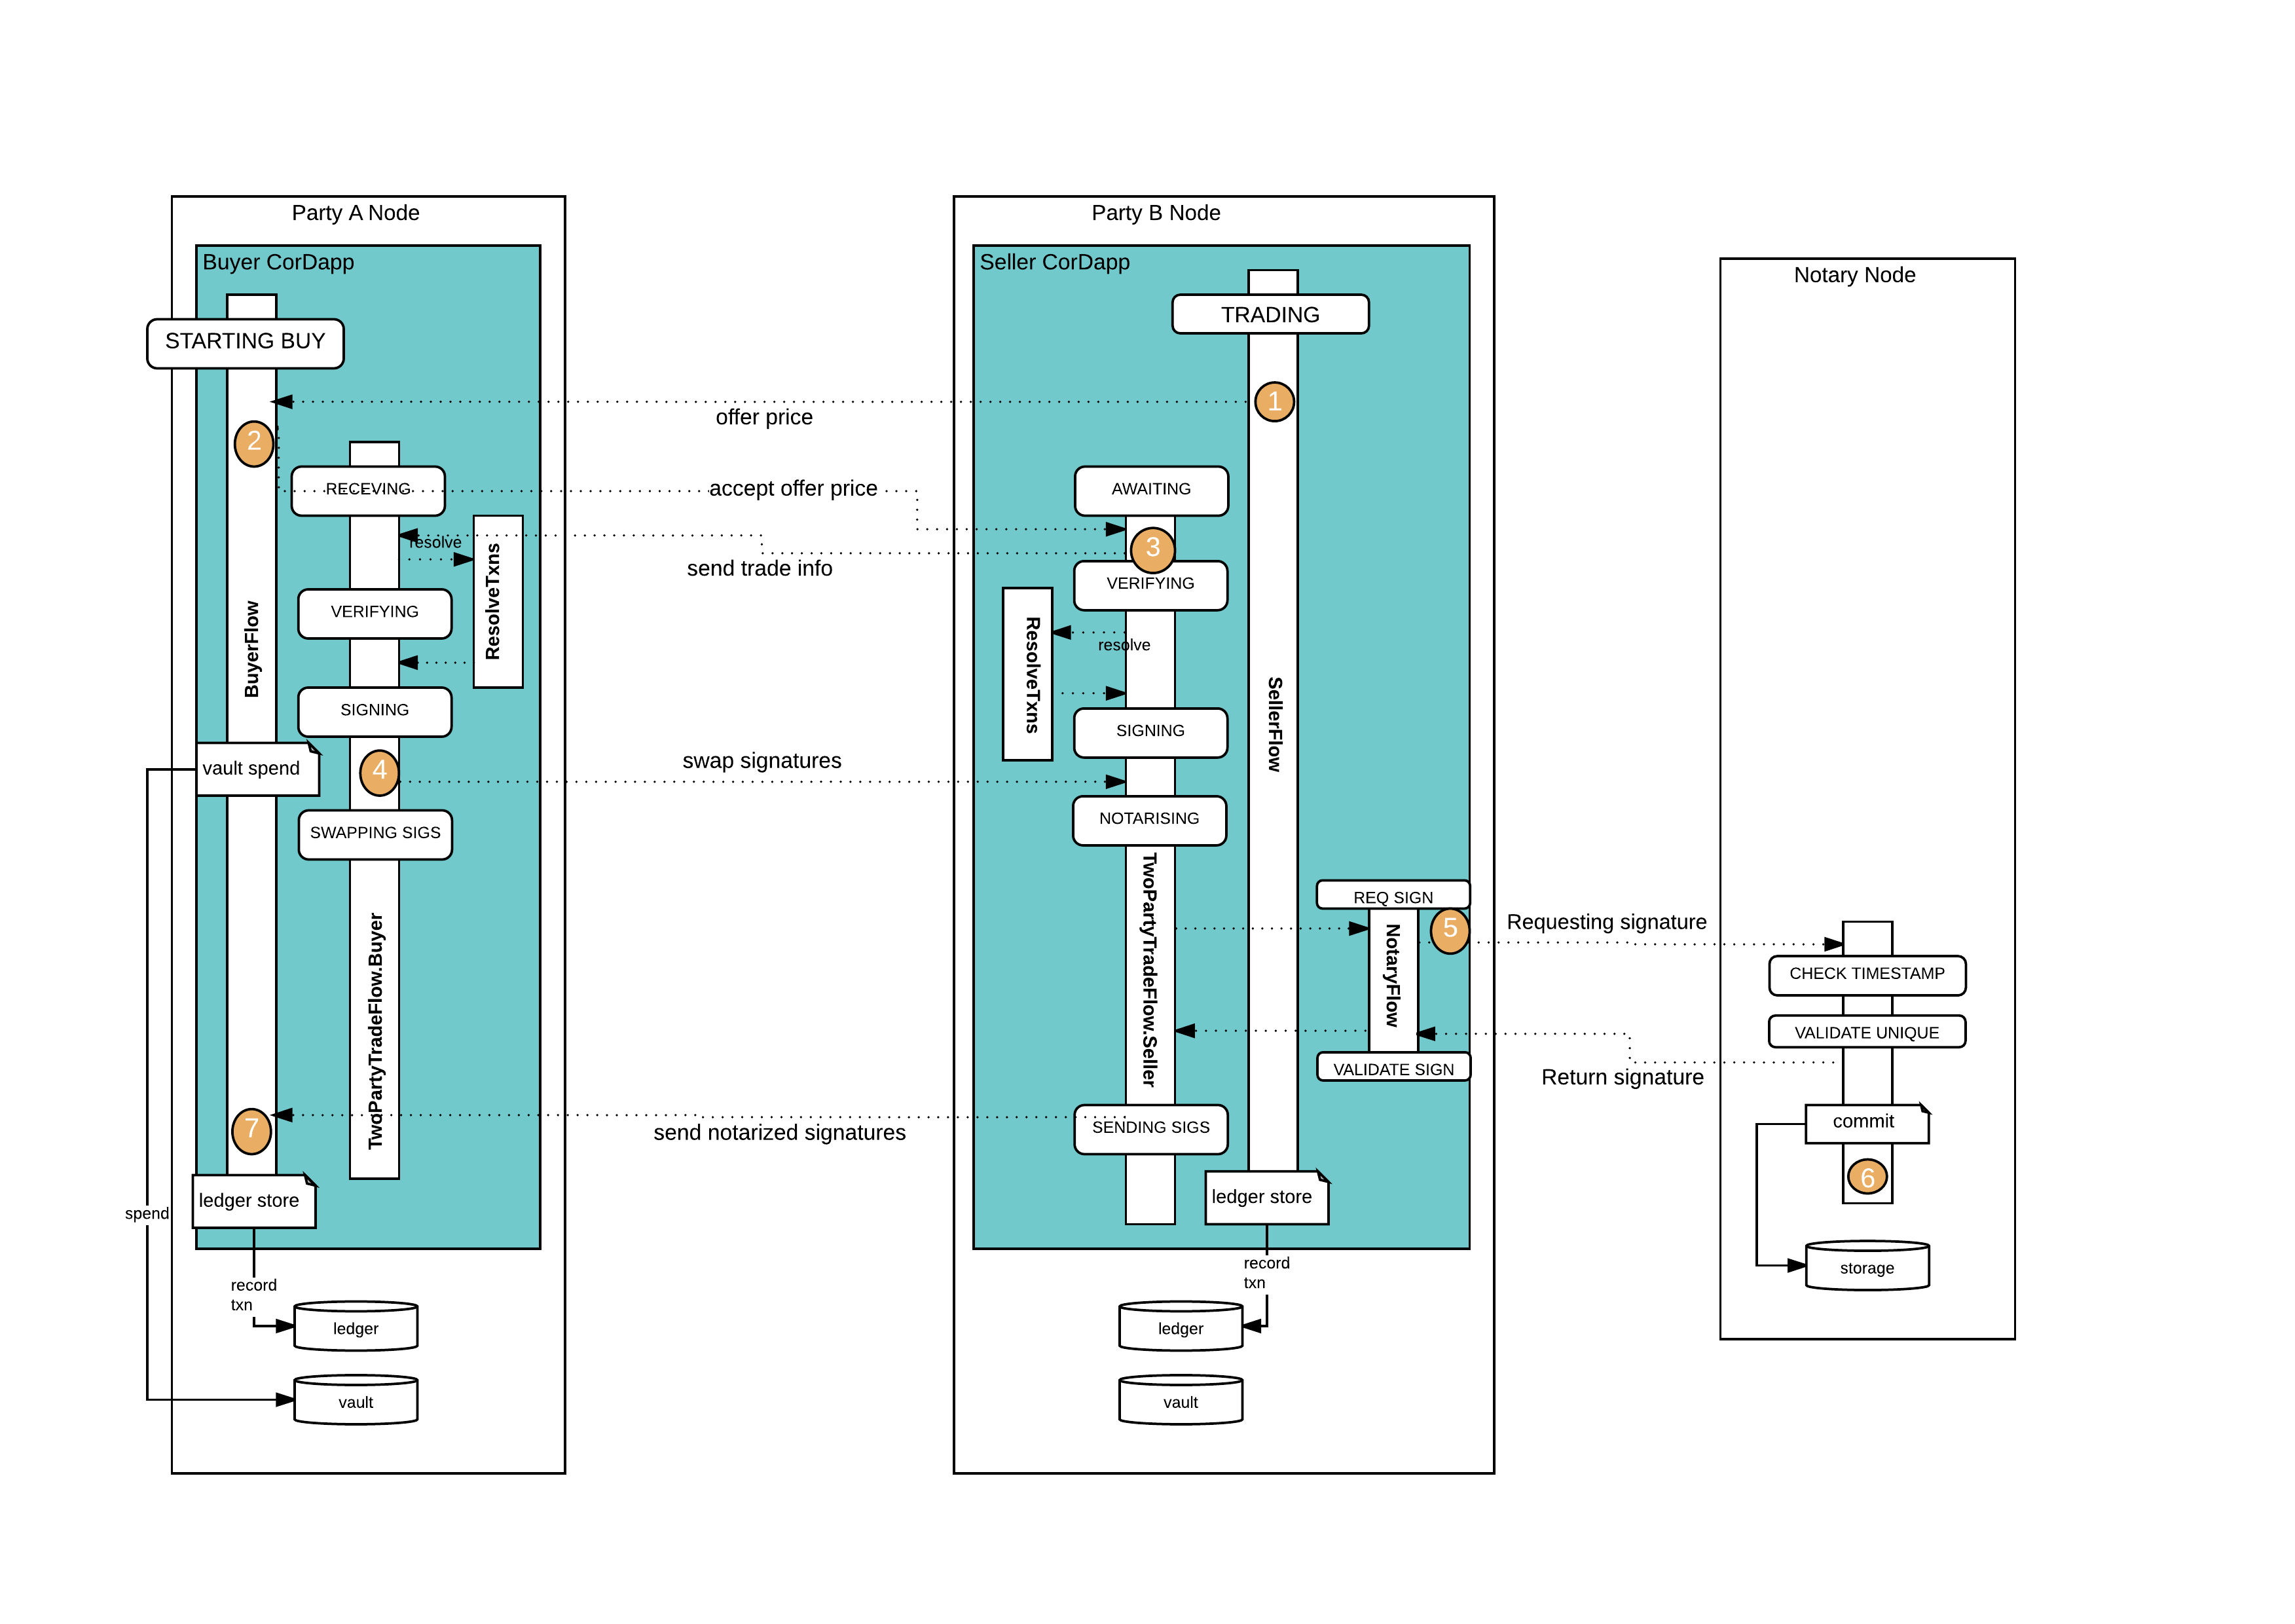
\includegraphics[scale=0.16, center]{trading-flow}
%\caption{A diagram showing the two party trading flow with notarisation}
%\end{figure}

\subsection{Data visibility and dependency resolution}\label{subsec:data-visibility-and-dependency-resolution}

When a transaction is presented to a node as part of a flow it may need to be checked. Simply sending you a message
saying that I am paying you \pounds1000 is only useful if you are sure I own the money I'm using to pay you.
Checking transaction validity is the responsibility of the \texttt{ResolveTransactions} flow. This flow performs a
breadth-first search over the transaction graph, downloading any missing transactions into local storage from the
counterparty, and validating them. The search bottoms out at the issuance transactions. A transaction is not
considered valid if any of its transitive dependencies are invalid.

It is required that a node be able to present the entire dependency graph for a transaction it is asking another
node to accept. Thus there is never any confusion about where to find transaction data and there is never any need
to reach out to dozens of nodes which may or may not be currently available. Because transactions are always
communicated inside a flow, and flows embed the resolution flow, the necessary dependencies are fetched and checked
automatically from the correct peer. Transactions propagate around the network lazily and there is no need for
distributed hash tables.

This approach has several consequences. One is that transactions that move highly liquid assets like cash may end
up becoming a part of a very long chain of transactions. The act of resolving the tip of such a graph can involve
many round-trips and thus take some time to fully complete. How quickly a Corda network can send payments is thus
difficult to characterise: it depends heavily on usage and distance between nodes. Whilst nodes could pre-push
transactions in anticipation of them being fetched anyway, such optimisations are left for future work.

Whilst this system is simpler than creating rigid data partitions and clearly provides better privacy than global
broadcast, in the absence of additional privacy measures it is nonetheless still difficult to reason about who may
get to see transaction data. This uncertainty is mitigated by several factors.

\paragraph{Small-subgraph transactions.}Some uses of the ledger do not involve widely circulated asset states. For
example, two institutions that wish to keep their view of a particular deal synchronised but who are making related
payments off-ledger may use transactions that never go outside the involved parties. A discussion of on-ledger vs
off-ledger cash can be found in a later section.

\paragraph{Transaction privacy techniques.}Corda supports a variety of transaction data hiding techniques. For
example, public keys can be randomised to make it difficult to link transactions to an identity. ``Tear-offs''
(\cref{sec:tear-offs}) allow some parts of a transaction to be presented without the others. In future versions of
the system secure hardware and/or zero knowledge proofs could be used to convince a party of the validity of a
transaction without revealing the underlying data.

\paragraph{State re-issuance.}In cases where a state represents an asset that is backed by a particular issuer, and
the issuer is trusted to behave atomically even when the ledger isn't forcing atomicity, the state can simply be
`exited' from the ledger and then re-issued. Because there are no links between the exit and reissue transactions
this shortens the chain. In practice most issuers of highly liquid assets are already trusted with far more
sensitive tasks than reliably issuing pairs of signed data structures, so this approach is unlikely to be an issue.

\section{Identity}\label{sec:identity}

In all decentralised ledger systems data access is controlled using asymmetric key pairs. Because public keys are
difficult for humans to reliably remember or write down, a naming layer is added on top based on X.509 certificate
hierarchies rooted at a single certificate authority for each network (see~\cref{subsec:the-identity-root}). This
is beneficial for security. Many large attacks on cryptocurrencies have exploited the fact that destination
addresses are raw (hashes of) public keys, thus all look the same and it's up to users or app developers to map
these to more natural forms. Phishing attacks, viruses that detect addresses being copied to the clipboard and
substitute them, hacks on web forums to replace addresses and more have all been reported. By allowing both
apps and users to work in terms of natural language identities, multiple avenues for attack are closed.

More complex notions of identity that may attest to many time-varying attributes are not handled at this layer of
the system: the base identity is always just an X.500 name. Note that even though messaging is always identified,
ledger data itself may contain anonymous public keys that aren't linked to any part of the network's PKI.

In most implementations, the network map will only agree to list nodes that have a valid identity certificate.
Because nodes will only accept connections from other nodes in the network map by default, this provides a form of
abuse control in which abusive parties can be evicted from the network. `Abuse' in this context has a technical
connotation, for example, mounting application level denial of service attacks, being discovered using a
fraudulently obtained identity or failing to meet network policy, for example by falling too far behind the
minimum required platform version.

The design attempts to constrain what malicious or compromised network operators can do.  A compromised network
operator may decide to delist a node for reasons that were not previously agreed to. Such an operator can be
overridden locally by providing signed \texttt{NodeInfo} files to a node, which would allow flows and transactions
to continue. It's possible that in future a way to override the identity root may also be provided.

An important point is that naming is only used for \emph{resolution} to public keys or IP addresses, however, names
are not \emph{required} for this resolution. They're just a convenience. The ledger is intended to contain resolved
public keys for access control purposes: this design creates an important limitation on the power of the naming
authority. Maliciously issuing a certificate binding a pre-existing name to a new key owned by the attacker doesn't
allow them to edit any of the existing data on the ledger, nor steal assets, as the states contain only keys which
cannot be changed after a state is created. This in turn implies that, like with all block chain systems, there's
no way to recover from losing your keys. A future version of the platform may add limited support for key rotation
by having both key owner and identity root sign a key change message, but the design does not anticipate ever
allowing the identity root to unilaterally re-assign identities to someone else.

An additional impact of this decision is that public keys can be discovered via alternate means and then used on
ledger. QR codes, Bluetooth discovery, alternate or even competing naming services and direct input are all
possible ways to obtain public keys.

\subsection{Hierarchical identity}\label{subsec:hierarchical-identity}

The peer-to-peer network is flat and requires that any node can directly connect to any other. However it would be
useful to extend the network to be multi-level, such that entities without nodes can nonetheless take part in a
limited way via a proxy or hosting node of some kind. This requires a way to identify these entities such that they
can be linked to their hosting node.

The certificate hierarchy is designed to create a flexible global namespace in which organisations, individuals,
devices and groups can all be bound to public keys. The standard web PKI uses X.509 path length constraints to
prevent holders of certificates issuing themselves more sub-certificates, but Corda uses X.509 name constraints to
enable sub-certificates. A holder of a certificate with a name like \texttt{C=US, S=CA, O=MegaCorp} (a company
called MegaCorp in California) can issue certificates for names with additional components, for example,
\texttt{C=US, S=CA, O=MegaCorp, CN=user@megacorp.com}. These components could reflect employees, account holders or
machines manufactured by the firm. Future versions of the flow framework will understand how to route flow sessions
based on these names via their controlling organisational nodes by simply finding the most precise match for the
name (after discarding suffixes) in the network map, thus enabling apps to start structured conversations with
those entities.

The identity hierarchy has a single root: the node's network operator. In effect there is only one root certificate
authority. This may appear different to the web PKI (in which there are many competing CAs) but is actually the
same. On the web, the identity hierarchy root is your browser or operating system vendor. These vendors select which
certificate authorities are a part of the `root store' and thus trusted to verify identities. Authority is ultimately
only delegated by the software vendors. Corda doesn't ship a root store, as that would make the software maintainers
be the ultimate identity root of all networks granting too much power. Consider a software update that added a CA
to the trust store controlled by a rogue developer, for example - this would grant that rogue developer full read/write
access to every Corda network.

Instead, the network operator is the root and may delegate authority as they see fit. Whilst normally used to
delegate authority over the sub-namespace of a single legal entity, as described above, it is theoretically also
possible to delegate in other ways, for example, along national boundaries, or simply to grant unconstrained
certificate-issuing power to other firms, as is done in the web PKI. In such a configuration care would have to be
taken to ensure only a single certificate laying claim to a name/key pair was issued, as the platform as this time
cannot handle the ambiguity of multiple live certificates for the same identity in different parts of the
hierarchy. The issues involved in having multiple certificate issuers for a single network may be addressed in
future work, but would not remove the requirement to have a single coherent set of network parameters.

\subsection{Confidential identities}\label{subsec:confidential-identities}

A standard privacy technique in block chain systems is the use of randomised unlinkable public keys to stand in for
actual verified identities. The platform allows an identity to be obfuscated on the ledger by generating keys not
linked anywhere in the PKI and then using them in the ledger. Ownership of these pseudonyms may be revealed to a
counterparty using a simple interactive protocol in which Alice selects a random nonce (`number used once') and
sends it to Bob, who then signs the nonce with the private key corresponding to the public key he is proving
ownership of. The resulting signature is then checked and the association between the anonymous key and the primary
identity key is recorded by the requesting node. This protocol is provided to application developers as a set of
subflows they can incorporate into their apps. Resolution of transaction chains thus doesn't reveal anything about
who took part in the transaction.

Generating fresh keys for each new deal or asset transfer rapidly results in many private keys being created. These
keys must all be backed up and kept safe, which poses a significant management problem when done at scale. The
canonical way to resolve this problem is through the use of deterministic key derivation, as pioneered by the
Bitcoin community in BIP 32 `Hierarchical Deterministic Wallets'\cite{BIP32}. Deterministic key derivation allows
all private key material needed to be derived from a single, small pool of entropy (e.g. a carefully protected and
backed up 128 bits of random data). More importantly, when the full BIP 32 technique is used in combination with an
elliptic curve that supports it, public keys may also be deterministically derived \emph{without} access to the
underlying private key material. This allows devices to provide fresh public keys to counterparties without being
able to sign with those keys, enabling better security along with operational efficiencies.

There are constraints on the mathematical properties of the digital signature algorithms parties use, and the
protocol signature algorithms for which deterministic derivation isn't possible. Additionally it's common for nodes
to keep their private keys in hardware security modules that may also not support deterministic derivation.
However, implementations are recommended to use hierarchical deterministic key derivation when possible.

% CODEME: The platform doesn't do suffix stripping at the moment.

\subsection{Accounts}\label{subsec:accounts}

The ability for nodes to use confidential identities isn't only useful for anonymising the node owner. It's
possible to locally mark anonymous keys with private, randomly generated \emph{universally unique identifiers}
(UUIDs). These UUIDs can be used for any purpose, but a typical use is to assign keys as owned by some node user
that isn't otherwise exposed to the ledger. The flow framework understands how to start a flow with a
confidential identity if the subflows discussed above have been used to establish ownership beforehand.

This feature must be used with care. There's no way for the private key to be held outside the node at the time
of writing and enabling non-node software to safely sign transactions requires some subtle enhancements
(see~\cref{sec:secure-signing-devices}). Moreover it's only reasonable to do this in specific situations, such
as when the signer of a transaction is an employee of the organisation hosting the node. This is because whilst
signing external to the node may reduce the impact of a compromised server the node itself still has full access
to all the data (account holder has no privacy from the node operator), and the node may mis-report
the contents of the ledger at any time. Thus the node still has considerable power, even in a situation where
the signing keys are no longer directly accessible.

\section{Data model}

\subsection{Transaction structure}\label{subsec:transaction-structure}

States are the atomic unit of information in Corda. They are never altered: they are either current (`unspent') or
consumed (`spent') and hence no longer valid.  Transactions read zero or more states (inputs), consume zero or more
of the read states, and create zero or more new states (outputs). Because states cannot exist outside of the
transactions that created them, any state whether consumed or not can be identified by the identifier of the
creating transaction and the index of the state in the outputs list.

A basic need is to represent pointers to data on the ledger. A \texttt{StateRef} type models the combination of a
transaction identifier and an output index. StateRefs can identify any piece of data on the ledger at any point in
its history in a compact, unified form. The \texttt{StatePointer} type unifies a standard JVM memory reference with
its cryptographic ledger counterpart. There are two kinds of pointer: static and linear. A static pointer is simply
a wrapped \texttt{StateRef} which can be easily resolved to the pointed-to state if it's available in the vault. A
linear pointer contains a UUID (universally unique identifier, a 128-bit random number) that identifies a chain of
\emph{linear states}. Linear states copy the UUID from input to output, thus allowing you to talk about the latest
version of a piece of data independent of its hash-based ledger coordinates.

Transactions consist of the following components:

\begin{labeling}{Input references}
\item [Consuming input references.] These are \texttt{(hash, output index)} pairs that point to the states a
transaction is consuming.
\item [Output states.] Each state specifies the notary for the new state, the contract(s) that define its allowed
transition functions and finally the data itself.
\item [Non-consuming input references.] These are also \texttt{(hash, output index)} pairs, however these `reference
states' are not consumed by the act of referencing them. Reference states are useful for importing data that gives
context to other states but which is only changed from time to time. Note that the pointed to state must be unconsumed
at the time the transaction is notarised: if it's been consumed itself as part of a different transaction, the referencing
transaction will not be notarised. In this way, non-consuming input references can help prevent the execution of
transactions that rely on out-of-date reference data.
\item [Attachments.] Transactions specify an ordered list of zip file hashes. Each zip file may contain
code and data for the transaction. Contract code has access to the contents of the attachments when checking the
transaction for validity. Attachments have no concept of `spentness' and are useful for things like holiday
calendars, timezone data, bytecode that defines the contract logic and state objects, and so on.
\item [Commands.] There may be multiple allowed output states from any given input state. For instance
an asset can be moved to a new owner on the ledger, or issued, or exited from the ledger if the asset has been
redeemed by the owner and no longer needs to be tracked. A command is essentially a parameter to the contract
that specifies more information than is obtainable from examination of the states by themselves (e.g. data from an oracle
service). Each command has an associated list of public keys. Like states, commands are object graphs. Commands therefore
define what a transaction \emph{does} in a conveniently accessible form.
\item [Signatures.] The set of required signatures is equal to the union of the commands' public keys. Signatures can use
a variety of cipher suites - Corda implements cryptographic agility.
\item [Type.] Transactions can either be normal, notary-changing or explicit upgrades. The validation rules for each are
different.
\item [Timestamp.] When present, a timestamp defines a time range in which the transaction is considered to
have occurred. This is discussed in more detail below.
\item [Network parameters.] Specifies the hash and epoch of the network parameters that were in force at the time the
transaction was notarised. See \cref{subsec:network-parameters} for more details.
% \item [Summaries] Textual summaries of what the transaction does, checked by the involved smart contracts. This field
% is useful for secure signing devices (see \cref{sec:secure-signing-devices}).
\end{labeling}

% TODO: This description ignores the participants field in states, because it probably needs a rethink.
% TODO: Summaries aren't implemented.

The platform provides a \texttt{TransactionBuilder} class which, amongst many other features, automatically
searches the object graph of each state and command to locate linear pointers, resolve them to the latest known
state and add that state as a non-consumed input, then searches the resolved state recursively. Note that the `latest' version is determined relative to an
individual node's viewpoint, thus, it may not be truly the latest version at the time the transaction is built. The
state's notary cluster will reject the transaction if this occurs, at which point the node may take some action to
discover the latest version of the state and try again.

Transactions are identified by the root of a Merkle tree computed over the components. The transaction format is
structured so that it's possible to deserialize some components but not others: a \emph{filtered transaction} is
one in which only some components are retained (e.g. the inputs) and a Merkle branch is provided that proves the
inclusion of those components in the original full transaction. We say these components have been `torn off'. This
feature is particularly useful for keeping data private from notaries and oracles. See~\cref{sec:tear-offs}.

Signatures are appended to the end of a transaction thus signature malleability as seen in the Bitcoin protocol is
not a problem. There is never a need to identify a transaction with its accompanying signatures by hash. Signatures
can be both checked and generated in parallel, and they are not directly exposed to contract code. Instead
contracts check that the set of public keys specified by a command is appropriate, knowing that the transaction
will not be valid unless every key listed in every command has a matching signature. Public key structures are
themselves opaque. In this way high performance through parallelism is possible and algorithmic agility is
retained. New signature algorithms can be deployed without adjusting the code of the smart contracts themselves.

This transaction structure is fairly complex relative to competing systems. The Corda data model is designed for
richness, evolution over time and high performance. The cost of this is that transactions have more components than
in simpler systems.

\begin{figure}[H]

\includegraphics[width=\textwidth]{cash}
\caption{An example of a cash issuance transaction}
\end{figure}

\paragraph{Example.}In the diagram above, we see an example of a cash issuance transaction. The transaction (shown
lower left) contains zero inputs and one output, a newly issued cash state. The cash state (shown expanded top
right) contains several important pieces of information: 1) details about the cash that has been issued -- amount,
currency, issuer, owner and so forth, 2) the contract code whose verify() function will be responsible for
verifying this issuance transaction and also any transaction which seeks to consume this state in the future, 3) a
hash of a document which may contain overarching legal prose to ground the behaviour of this state and its contract
code in a governing legal context.

The transaction also contains a command, which specifies that the intent of this transaction is to issue cash and
the command specifies a public key. The cash state's verify function is responsible for checking that the public
key(s) specified on the command(s) are those of the parties whose signatures would be required to make this
transaction valid. In this case, it means that the verify() function must check that the command has specified a
key corresponding to the identity of the issuer of the cash state. The Corda framework is responsible for checking
that the transaction has been signed by all keys listed by all commands in the transaction. In this way, a verify()
function only needs to ensure that all parties who need to sign the transaction are specified in commands, with the
framework responsible for ensuring that the transaction has been signed by all parties listed in all commands.

\subsection{Composite keys}\label{sec:composite-keys}

The term ``public key'' in the description above actually refers to a \emph{composite key}. Composite keys are
trees in which leaves are regular cryptographic public keys with an accompanying algorithm identifiers. Nodes in
the tree specify both the weights of each child and a threshold weight that must be met. The validity of a set of
signatures can be determined by walking the tree bottom-up, summing the weights of the keys that have a valid
signature and comparing against the threshold. By using weights and thresholds a variety of conditions can be
encoded, including boolean formulas with AND and OR.

\begin{figure}[H]
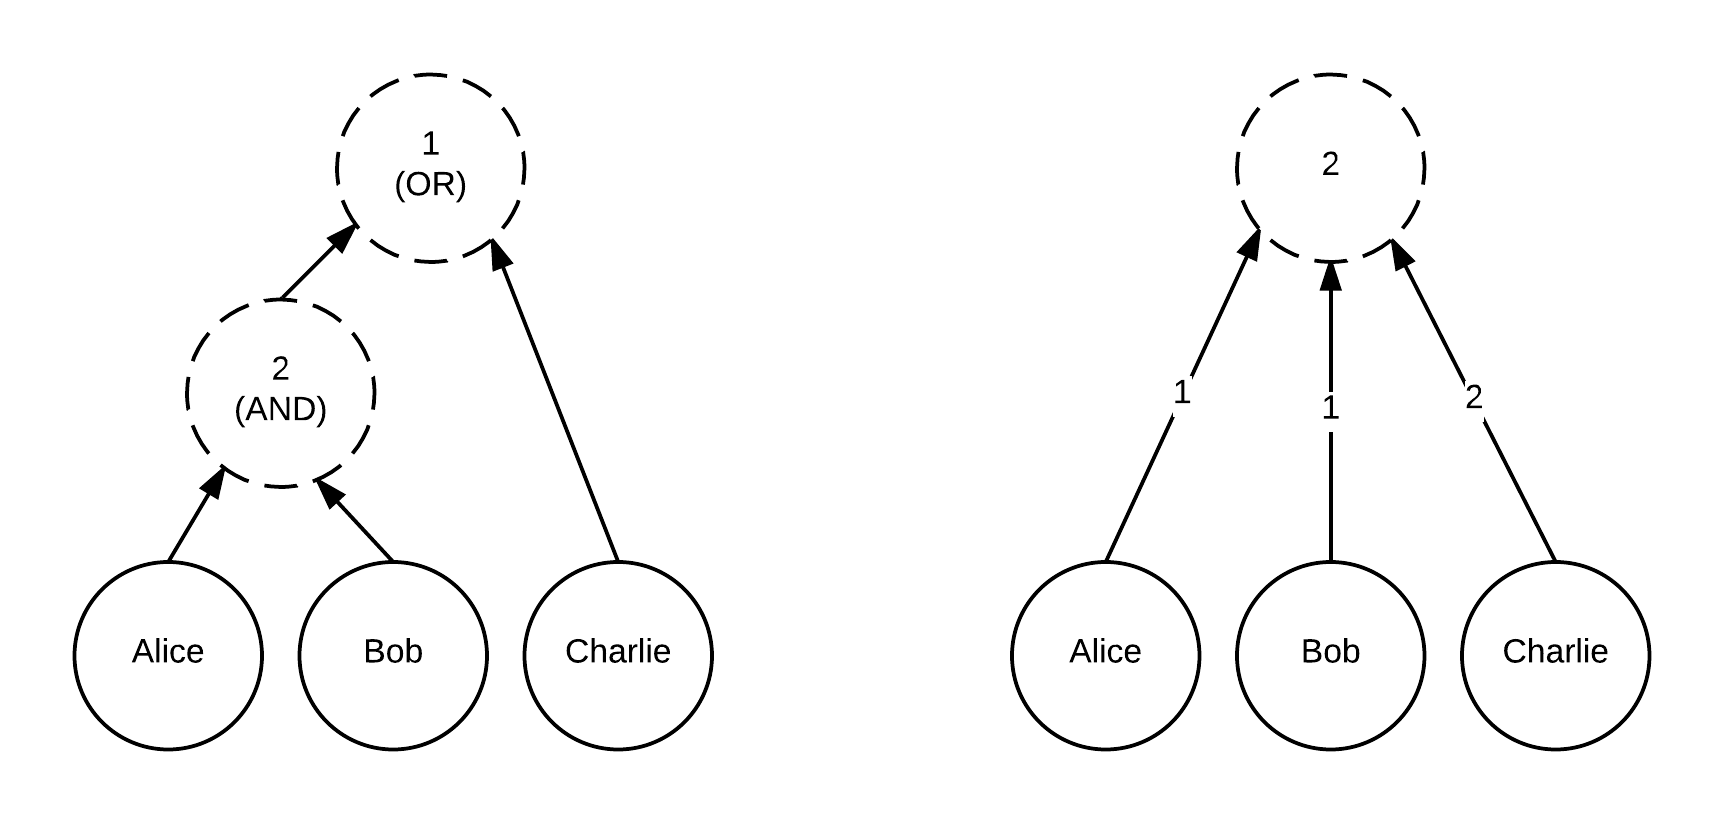
\includegraphics[width=\textwidth]{composite-keys}
\caption{Examples of composite keys}
\end{figure}

Composite keys are useful in multiple scenarios. For example, assets can be placed under the control of a 2-of-2
composite key where one leaf key is owned by a user, and the other by an independent risk analysis system. The risk
analysis system refuses to sign if the transaction seems suspicious, like if too much value has been transferred in
too short a time window. Another example involves encoding corporate structures into the key, allowing a CFO to
sign a large transaction alone but his subordinates are required to work together.

Composite keys are also useful for byzantine fault tolerant notaries. Each participant in a distributed notary is
represented by a leaf, and the threshold is set such that some participants can be offline or refusing to sign yet
the signature of the group is still valid.

Whilst there are threshold signature schemes in the literature that allow composite keys and signatures to be
produced mathematically, we choose the less space efficient explicit form in order to allow a mixture of keys using
different algorithms. In this way old algorithms can be phased out and new algorithms phased in without requiring
all participants in a group to upgrade simultaneously.

\subsection{Time handling}\label{sec:timestamps}

Transaction timestamps specify a \texttt{[start, end]} time window within which the transaction is asserted to have
occurred. Timestamps are expressed as windows because in a distributed system there is no true time, only a large
number of desynchronised clocks. This is not only implied by the laws of physics but also by the nature of shared
transactions - especially if the signing of a transaction requires multiple human authorisations, the process of
constructing a joint transaction could take hours or even days.

It is important to note that the purpose of a transaction timestamp is to communicate the transaction's position on
the timeline to the smart contract code for the enforcement of contractual logic. Whilst such timestamps may also
be used for other purposes, such as regulatory reporting or ordering of events in a user interface, there is no
requirement to use them like that and locally observed timestamps may sometimes be preferable even if they will not
exactly match the time observed by other parties. Alternatively if a precise point on the timeline is required and
it must also be agreed by multiple parties, the midpoint of the time window may be used by convention. Even though
this may not precisely align to any particular action (like a keystroke or verbal agreement) it is often useful
nonetheless.

Timestamp windows may be open ended in order to communicate that the transaction occurred before a certain time or
after a certain time, but how much before or after is unimportant. This can be used in a similar way to Bitcoin's
\texttt{nLockTime} transaction field, which specifies a \emph{happens-after} constraint.

Timestamps are checked and enforced by notary services. As the participants in a notary service will themselves not
have precisely aligned clocks, whether a transaction is considered valid or not at the moment it is submitted to a
notary may be unpredictable if submission occurs right on a boundary of the given window. However, from the
perspective of all other observers the notary's signature is decisive: if the signature is present, the transaction
is assumed to have occurred within that time.

\paragraph{Reference clocks.}In order to allow for relatively tight time windows to be used when transactions are
fully under the control of a single party, notaries are expected to be synchronised to international atomic time
(TIA). Accurate feeds of this clock can be obtained from GPS satellites and long-wave radio. Note that Corda uses
the Google/Amazon timeline, which is UTC with a leap smear from noon to noon across the leap event, thus each day
always has exactly 86400 seconds.

\paragraph{Timezones.}Business agreements typically specify times in local time zones rather than offsets from
midnight UTC on January 1st 1970, although the latter would be more civilised. Because the Corda type system is the
Java type system, developers can embed \texttt{java.time.ZonedDateTime} in their states to represent a time
specified in a specific time zone. This allows ensure correct handling of daylight savings transitions and timezone
definition changes. Future versions of the platform will allow timezone data files to be attached to transactions,
to make such calculations entirely deterministic.

\subsection{Attachments and contract bytecodes}\label{subsec:attachments-and-contract-bytecodes}

Transactions may have a number of \emph{attachments}, identified by the hash of the file. Attachments are stored
and transmitted separately to transaction data and are fetched by the standard resolution flow only when the
attachment has not previously been seen before.

Attachments are always zip files\cite{ZipFormat}. The files within the zips are collapsed together into a single
logical file system and class path.

Smart contracts in Corda are defined using a restricted form of JVM bytecode as specified in \emph{``The Java
Virtual Machine Specification SE 8 Edition''}\cite{JVM}, with some small differences that are described in a later
section. A contract is simply a class that implements the \texttt{Contract} interface, which in turn exposes a
single function called \texttt{verify}. The verify function is passed a transaction and either throws an exception
if the transaction is considered to be invalid, or returns with no result if the transaction is valid. The set of
verify functions to use is the union of the contracts specified by each state, which are expressed as a class name
combined with a \emph{constraint} (see~\cref{sec:contract-constraints}). Embedding the JVM specification in the
Corda specification enables developers to write code in a variety of languages, use well developed toolchains, and
to reuse code already authored in Java or other JVM compatible languages. A good example of this feature in action
is the ability to embed the ISDA Common Domain Model\cite{ISDACDM} directly into CorDapps. The CDM is
a large collection of types mapped to Java classes that model derivatives trading in a standardised way. It is
common for industry groups to define such domain models and for them to have a Java mapping.

Current versions of the platform only execute attachments that have been previously installed (and thus
whitelisted), or attachments that are signed by the same signer as a previously installed attachment. Thus nodes
may fail to reach consensus on long transaction chains that involve apps your counterparty has not seen. Future
versions of the platform will run contract bytecode inside a deterministic JVM. See~\cref{sec:djvm}.

The Java standards also specify a comprehensive type system for expressing common business data. Time and calendar
handling is provided by an implementation of the JSR 310 specification, decimal calculations can be performed
either using portable (`\texttt{strictfp}') floating point arithmetic or the provided bignum library, and so on.
These libraries have been carefully engineered by the business Java community over a period of many years and it
makes sense to build on this investment.

Contract bytecode also defines the states themselves, which may be directed acyclic object graphs. States may label
their properties with a small set of standardised annotations. These can be useful for controlling how states are
serialized to JSON and XML (using JSR 367 and JSR 222 respectively), for expressing static validation constraints
(JSR 349) and for controlling how states are inserted into relational databases (JSR 338). This feature is
discussed later. Future versions of the platform may additionally support cyclic object graphs.

\paragraph{Data files.}Attachments may also contain data files that support the contract code. These may be in the
same zip as the bytecode files, or in a different zip that must be provided for the transaction to be valid.
Examples of such data files might include currency definitions, timezone data and public holiday calendars. Any
public data may be referenced in this way. Attachments are intended for data on the ledger that many parties may
wish to reuse over and over again. Data files are accessed by contract code using the same APIs as any file on the
classpath would be accessed. The platform imposes some restrictions on what kinds of data can be included in
attachments along with size limits, to avoid people placing inappropriate files on the global ledger (videos,
PowerPoints etc).

Note that the creator of a transaction gets to choose which files are attached. Therefore, it is typical that
states place constraints on the application JARs they're willing to accept. This enables the software that imposes
logic on the ledger to evolve independently of the stored data, whilst still remaining secure against malicious
evolutions that would, for example, allow an adversary to print money. These mechanisms are discussed
in~\cref{sec:contract-constraints}.

\paragraph{Signing.}Attachments may be signed using the JAR signing standard. No particular certificate is
necessary for this: Corda accepts self signed certificates for JARs. The signatures are useful for two purposes.
Firstly, it allows states to express that they can be satisfied by any attachment signed by a particular provider.
This allows on-ledger code to be upgraded over time. And secondly, signed JARs may provide classes in
`\emph{claimed packages}', which are discussed below.

\subsection{Contract constraints}\label{sec:contract-constraints}

In Bitcoin contract logic is embedded inside every transaction. Programs are small and data is inlined into the
bytecode, so upgrading code that's been added to the ledger is neither possible nor necessary. There's no need for
a mechanism to tie code and data together. In Corda contract logic may be far more complex. It will usually reflect
a changing business world which means it may need to be upgraded from time to time.

The easiest way of tying states to the contract code that defines them is by hash. This is equivalent to other
ledger platforms and is referred to as an \emph{hash constraint}. They work well for very simple and stable
programs, but more complicated contracts may need to be upgraded. In this case it may be preferable for states to
refer to contracts by the identity of the signer (a \emph{signature constraint}). Because contracts are stored in
zip files, and because a Java Archive (JAR) file is just a zip with some extra files inside, it is possible to use
the standard JAR signing infrastructure to identify the source of contract code. Simple constraints such as ``any
contract of this name signed by these keys'' allow for some upgrade flexibility, at the cost of increased exposure
to rogue contract developers. Requiring combinations of signatures helps reduce the risk of a rogue or hacked
developer publishing a bad contract version, at the cost of increased difficulty in releasing new versions. State
creators may also specify third parties they wish to review contract code. Regardless of which set of tradeoffs is
chosen, the framework can accommodate them.

A contract constraint may use a composite key of the type described in~\cref{sec:composite-keys}. The standard JAR
signing protocol allows for multiple signatures from different private keys, thus being able to satisfy composite
keys. The allowed signing algorithms are \texttt{SHA256withRSA} and \texttt{SHA256withECDSA}. Note that the
cryptographic algorithms used for code signing may not always be the same as those used for transaction signing, as
for code signing we place initial focus on being able to re-use the infrastructure.

\subsection{Precise naming}\label{subsec:precise-naming}

In any system that combines typed data with potentially malicious adversaries, it's important to always ensure
names are not allowed to become ambiguous or mixed up. Corda achieves this via a combination of different features.

\paragraph{No overlap rule.}Within a transaction attachments form a Java classpath. Class names are resolved by
locating the defining class file within the set of attachments and loading them via the deterministic JVM.
Unfortunately, out of the box Java allows different JAR files to define the same class name. Whichever JAR happens
to come first on the classpath is the one that gets used, but conventionally a classpath is not meant to have an
important ordering. This problem is a frequent source of confusion and bugs in Java software, especially when
different versions of the same module are combined into one program. On the ledger an adversary can craft a
malicious transaction that attempts to trick a node or application into thinking it does one thing whilst actually
doing another. To prevent attackers from building deliberate classpath conflicts to change the behaviour of code, a
transaction in which two file paths overlap between attachments is invalid. A small number of files that are
expected to overlap normally, such as files in the \texttt{META-INF} directory, are excluded.

\paragraph{Package namespace ownership.}Corda allows parts of the Java package namespace to be reserved for
particular developers with a network, identified by a public key (which may or may not be linked to an identity). Any JAR
that exports a class in an owned package namespace but which is not signed by the owning key is considered to be
invalid. Reserving a package namespace is optional but can simplify the data model and make applications more
secure.

The reason for this is related to a mismatch between the way the ledger names code and the way programming
languages do. In the distributed ledger world a bundle of code is referenced by hash or signing key, but in source
code English-like module names are used. In the Java ecosystem these names are broken into components separated by
dots, and there's a strong convention that names are chosen to start with the reversed domain name of the
developer's website. For example a developer who works for MegaCorp may use
\texttt{com.megacorp.superproduct.submodule} as a prefix for the names used in that specific product and submodule.

However this is only a convention. Nothing prevents anyone from publishing code that uses MegaCorp's package
namespace. Normally this isn't a problem as developers learn the correct names via some secure means, like browsing
an encrypted website of good reputation. But on a distributed ledger data can be encountered which was crafted by a
malicious adversary, usually a trading partner who hasn't been extensively verified or who has been compromised.
Such an adversary could build a transaction with a custom state and attachment that defined classes with the same
name as used by a real app. Whilst the core ledger can differentiate between the two applications, if data is
serialized or otherwise exposed via APIs that rely on ordinary types and class names the hash or signer of the
original attachment can easily get lost.

For example, if a state is serialized to JSON at any point then \emph{any} type that has the same shape can appear
legitimate. In Corda serialization types are ultimately identified by class name, as is true for all other forms of
serialization. Thus deserializing data and assuming the data represents a state only reachable by the contract
logic would be risky if the developer forgot to check that the original smart contract was the intended contract
and not one violating the naming convention.

By enforcing the Java naming convention cryptographically and elevating it to the status of a consensus rule,
developers can assume that a \texttt{com.megacorp.superproduct.DealState} type always obeys the rules enforced by
the smart contract published by that specific company. They cannot get confused by a mismatch between the human
readable self-assigned name and the cryptographic but non-human readable hash or key based name the ledger really
uses.

% TODO: Discuss confidential identities.
% TODO: Discuss the crypto suites used in Corda.

\subsection{Bug fixes and dispute resolution}\label{subsec:bug-fixes-and-dispute-resolution}

Decentralised ledger systems often differ in their underlying political ideology as well as their technical
choices. The Ethereum project originally promised ``unstoppable apps'' which would implement ``code as law''. After
a prominent smart contract was hacked\cite{TheDAOHack}, an argument took place over whether what had occurred could
be described as a hack at all given the lack of any non-code specification of what the program was meant to do. The
disagreement eventually led to a split in the community.

As Corda contracts are simply zip files, it is easy to include a PDF or other documents describing what a contract
is meant to actually do. A \texttt{@LegalProseReference} annotation is provided which by convention contains a URL
or URI to a specification document. There is no requirement to use this mechanism, and there is no requirement that
these documents have any legal weight. However in financial use cases it's expected that they would be legal
contracts that take precedence over the software implementations in case of disagreement.

It is technically possible to write a contract that cannot be upgraded. If such a contract governed an asset that
existed only on the ledger, like a cryptocurrency, then that would provide an approximation of ``code as law''. We
leave discussion of the wisdom of this concept to political scientists and reddit.

% TODO: Rewrite the section on confidential identities and move it under a new privacy section.

\subsection{Oracles and tear-offs}\label{sec:tear-offs}

It is sometimes convenient to reveal a small part of a transaction to a counterparty in a way that allows them to
both check and create signatures over the entire transaction. One typical use case for this is an \emph{oracle},
defined as a network service that is trusted to sign transactions containing statements about the world outside the
ledger only if the statements are true. Another use case is to outsource signing to small devices that can't or
won't process the entire transaction, which can potentially get very large for multi-party transactions. To make
this safe additional infrastructure is required, described in~\cref{sec:secure-signing-devices}.

Here are some example statements an oracle might check:

\begin{itemize}
\item The price of a stock at a particular moment was X.
\item An agreed upon interest rate at a particular moment was Y.
\item If a specific organisation has declared bankruptcy.
\item Weather conditions in a particular place at a particular time.
\end{itemize}

It is worth asking why a smart contract cannot simply fetch this information from some internet server itself: why
do we insist on this notion of an oracle. The reason is that all calculations on the ledger must be deterministic.
Everyone must be able to check the validity of a transaction and arrive at exactly the same answer, at any time
(including years into the future), on any kind of computer. If a smart contract could do things like read the
system clock or fetch arbitrary web pages then it would be possible for some computers to conclude a transaction
was valid, whilst others concluded it was not (e.g. if the remote server had gone offline). Solving this problem
means all the data needed to check the transaction must be in the ledger, which in turn implies that we must accept
the point of view of some specific observer. That way there can be no disagreement about what happened.

One way to implement oracles would be to have them sign a small data structure which is then embedded somewhere in
a transaction (in a state or command). We take a different approach in which oracles sign the entire transaction,
and data the oracle doesn't need to see is ``torn off'' before the transaction is sent. This is done by structuring
the transaction as a Merkle hash tree so that the hash used for the signing operation is the root. By presenting a
counterparty with the data elements that are needed along with the Merkle branches linking them to the root hash,
as seen in the diagrams below, that counterparty can sign the entire transaction whilst only being able to see some
of it. Additionally, if the counterparty needs to be convinced that some third party has already signed the
transaction, that is also straightforward. Typically an oracle will be presented with the Merkle branches for the
command or state that contains the data, and the timestamp field, and nothing else. If an oracle also takes part
in the ledger as a direct participant it should therefore derive a separate key for oracular usage, to avoid
being tricked into blind-signing a transaction that might also affect its own states.

\begin{figure}[H]
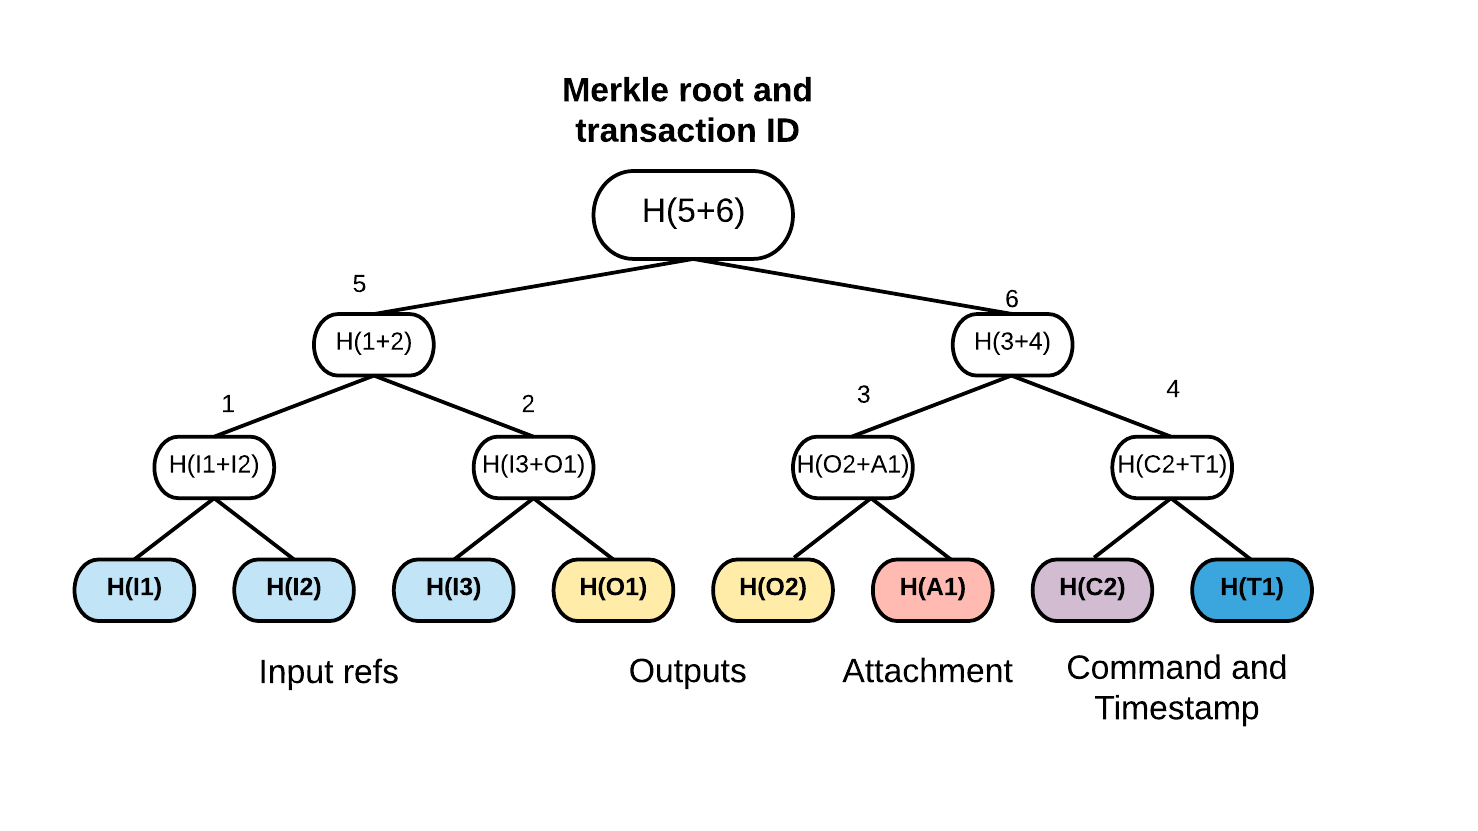
\includegraphics[width=\textwidth]{tearoffs1}
\caption{How the transaction's identifier hash is calculated}
\end{figure}

\begin{figure}[H]
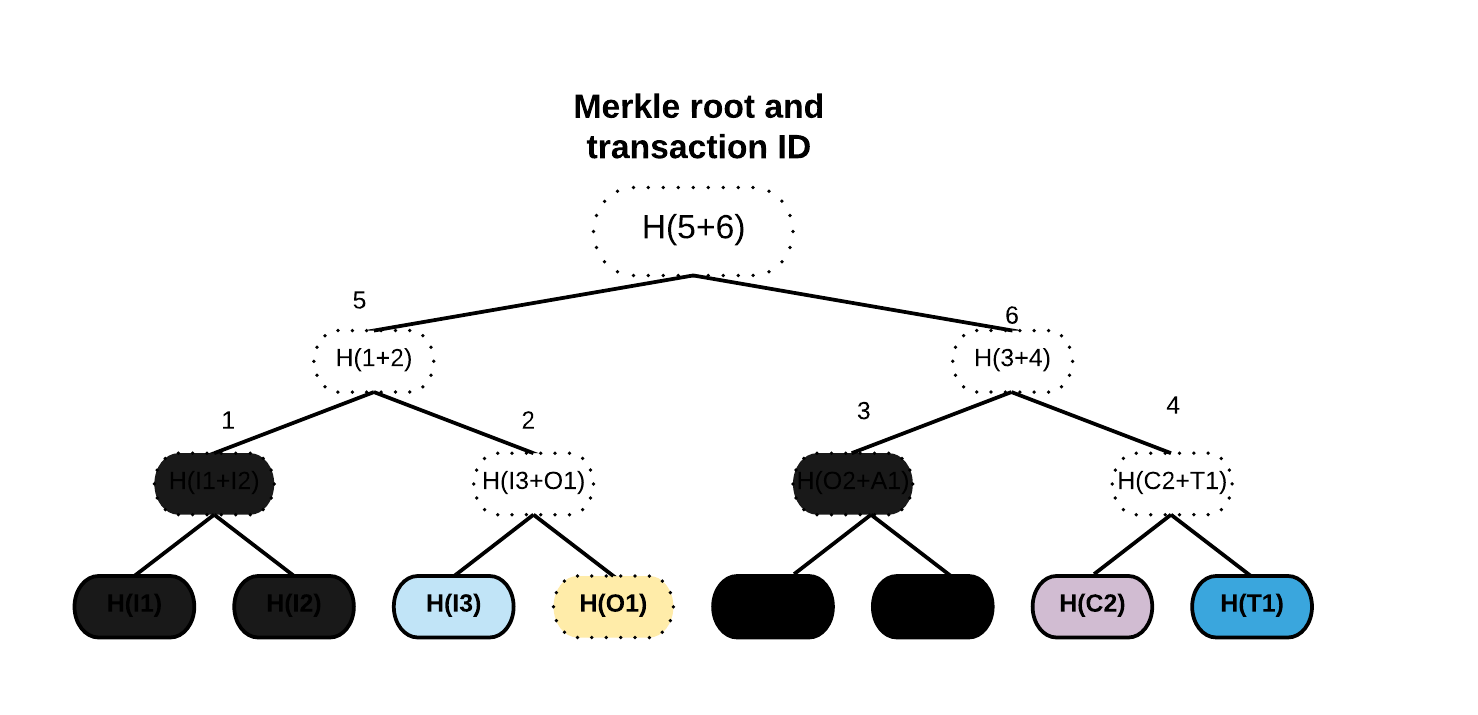
\includegraphics[width=\textwidth]{tearoffs2}
\caption{Construction of a Merkle branch}
\end{figure}

There are several reasons to take this more indirect approach. One is to keep a single signature checking code
path. By ensuring there is only one place in a transaction where signatures may be found, algorithmic agility and
parallel/batch verification are easy to implement. When a signature may be found in any arbitrary location in a
transaction's data structures, and where verification may be controlled by the contract code itself (as in
Bitcoin), it becomes harder to maximise signature checking efficiency. As signature checks are often one of the
slowest parts of a block chain system, it is desirable to preserve these capabilities.

Another reason is to provide oracles with a business model. If oracles just signed statements and nothing else then
it would be difficult to run an oracle in which there are only a small number of potential statements, but
determining their truth is very expensive. People could share the signed statements and reuse them in many
different transactions, meaning the cost of issuing the initial signatures would have to be very high, perhaps
unworkably high. Because oracles sign specific transactions, not specific statements, an oracle that is charging
for its services can amortise the cost of determining the truth of a statement over many users who cannot then
share the signature itself (because it covers a one-time-use structure by definition).

A final reason is that by signing transactions, the signature automatically covers the embedded time window, as
discussed in~\cref{sec:timestamps}. This provides a theoretically robust method of anchoring the oracle's statement
into the ledger's timeline.

\subsection{Encumbrances}\label{sec:encumbrances}

Each state in a transaction specifies a contract (boolean function) that is invoked with the entire transaction as
input. All contracts must accept in order for the transaction to be considered valid. Sometimes we would like to
compose the behaviours of multiple different contracts. Consider the notion of a ``time lock'' -- a restriction on
a state that prevents it being modified (e.g. sold) until a certain time. This is a general piece of logic that
could apply to many kinds of assets. Whilst such logic could be implemented in a library and then called from every
contract that might want to benefit from it, that requires all contract authors to think ahead and include the
functionality. It would be better if we could mandate that the time lock logic ran along side the contract that
governs the locked state.

Consider an asset that is supposed to remain frozen until a time is reached. Encumbrances allow a state to specify
another state that must be present in any transaction that consumes it. For example, a time lock contract can
define a state that contains the time at which the lock expires, and a simple contract that just compares that time
against the transaction timestamp. The asset state can be included in a spend-to-self transaction that doesn't
change the ownership of the asset but does include a time lock state in the outputs. Now if the asset state is
used, the time lock state must also be used, and that triggers the execution of the time lock contract.

Encumbered states can only point to one encumbrance state, but that state can itself point to another and so on,
resulting in a chain of encumbrances all of which must be satisfied.

% TODO: Diagram for how this is arranged

An encumbrance state must be present in the same transaction as the encumbered state, as states refer to each other
by index alone.

% TODO: Interaction of enumbrances with notary change transactions.

\subsection{Event scheduling}\label{sec:event-scheduling}

State classes may request flows to be started at given times. When a state is considered relevant by the vault and
the implementing CorDapp is installed and whitelisted by the administrator, the node may react to the passage of
time by starting new interactions with other nodes, people, or internal systems. As financial contracts often have
a notion of time in them this feature can be useful for many kinds of state transitions, for example, expiry of an
option contract, management of a default event, re-fixing of an interest rate swap and so on.

To request scheduled events, a state may implement the \texttt{SchedulableState} interface and then return a
request from the \texttt{nextScheduledActivity} function. The state will be queried when it is committed to the
vault and the scheduler will ensure the relevant flow is started at the right time.

\subsection{Tokens}\label{sec:tokens}

Some basic concepts occur in many kinds of application, regardless of what industry or use case it is for. The
platform provides a comprehensive type system for modelling of \emph{tokens}: abstract countable objects highly
suited to representing value.

Tokens can be used to model agreements with an issuer, like fiat money, securities, derivatives, debts and
other financial instruments. They could also  be used to model any sort of claim on physical resources,
like CPU time, network bandwidth, barrels of oil and so on. Finally, as a special case tokens can be used to
implement cryptocurrencies (this is modelled as a claim on a null issuer).

We define the notion of an \texttt{OwnableState}, implemented as an interface which any state may conform to.
Ownable states are required to have an \texttt{owner} field which is a composite key
(see~\cref{sec:composite-keys}). This is utilised by generic code in the vault (see~\cref{sec:vault}) to manipulate
ownable states.

From \texttt{OwnableState} we derive a \texttt{FungibleState} concept to represent an aggregation in which units
are sufficiently similar to be represented together in a single ledger state. Making that concrete, pound notes are
a fungible asset: regardless of whether you represent \pounds10 as a single \pounds10 note or two notes of \pounds5
each the total value is the same. Other kinds of fungible asset could be barrels of Brent Oil (but not all kinds of
crude oil worldwide, because oil comes in different grades which are not interchangeable), litres of clean water,
kilograms of bananas, units of a stock and so on.

Quantities are represented with an \texttt{Amount<T>} type which defines an integer amount parameterised by some
other type, usually a singleton object. To support tokens that have a fractional part, as some national currencies
do, the ``display token size'' is tracked explicitly. \texttt{Amount<T>} provides operator overloads to allow
addition, subtraction and multiplication with safety checks to prevent different tokens being combined together and
to catch integer overflow/underflow. These conditions normally indicate a programmer error or attack attempt.
Amounts may not be negative as in many critical contexts a negative quantity is undefined and reachable only
through an error condition. Transfers of value are modelled explicitly with an \texttt{AmountTransfer} type that
encodes direction.

\paragraph{Token SDK.}On top of these universal core types, Corda provides a dedicated `token software development
kit' module that  extends the type system with more sophisticated concepts.

\begin{figure}[H]
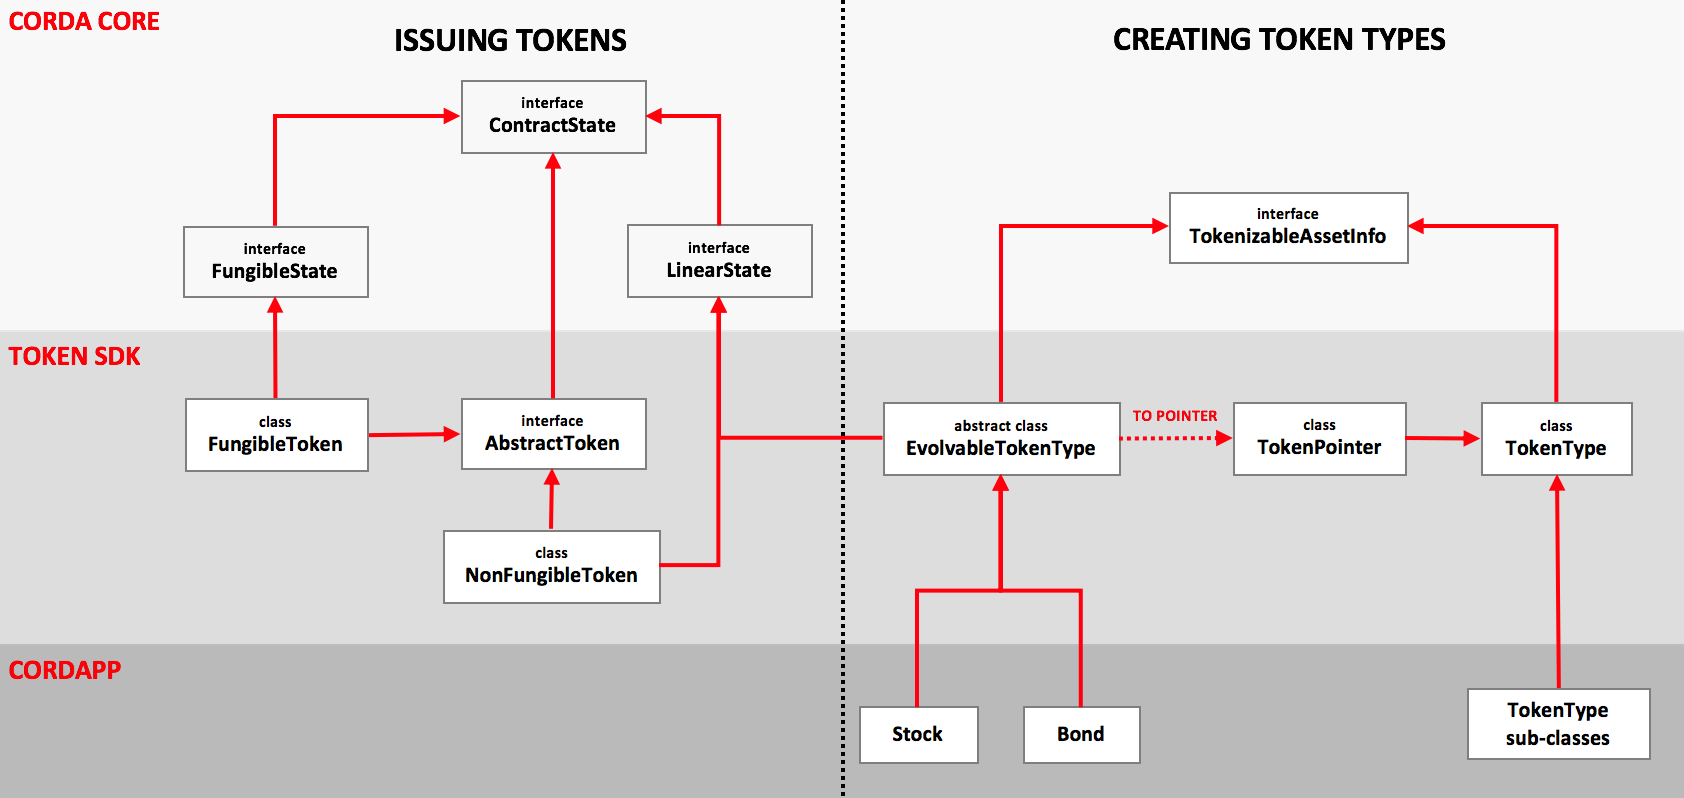
\includegraphics[width=\textwidth]{state-class-hierarchy}
\caption{Class hierarchy diagram showing the relationships between different state types}
\end{figure}

\texttt{TokenType} refers to a ``type of thing'' as opposed to the vehicle which is used to assign units of a token
to a particular owner. For that we use the \texttt{NonFungibleToken} state for assigning non-fungible tokens to a
holder and the \texttt{FungibleToken} state for assigning amounts of some fungible token to a holder. Because
tokens frequently represent claims on an issuer the \texttt{IssuedTokenType} class links a token type with an
issuing party. Whilst static token types never change, an \texttt{EvolvableTokenType} is an abstract linear state
that contains data defining the rules of the token or reference data related to it. For example a token type
representing a stock may include various metadata about that stock, such as regional identifiers. Token states are
linked to their defining token type states (when evolvable) using linear pointers
(see~\cref{subsec:transaction-structure}). This enables reference data about a token to be evolved such that
everyone always uses the latest version, ensuring a `golden source'. The lack of such global yet evolvable
definitions is a frequent problem in industry. Tokens with an issuer are \emph{not} fungible with each other: two
pools of pound sterling are considered to be separate types of token if they come from different issuers. This is
to avoid commingling and losing track of counterparty risk.

The token SDK provides APIs and flows to do standard tasks for UTXO based ledgers, such as moving tokens between
parties, issuing tokens, updating the definition of an evolvable token and efficient coin selection. This is the
task of selecting a group of states from the vault that add up to a certain value whilst minimising fragmentation,
transaction size and optimising other desirable characteristics. Although the term ``coin selection'' is an
anachronistic holdover from Bitcoin, Corda continues to use it due to the wealth of published literature exploring
algorithms for the task under this name.

Together, this functionality provides Corda's equivalent of the Ethereum ERC-20 standard\cite{ERC20}.

Having defined various kinds of abstract token, the SDK goes on to define (finally!) \texttt{Money} and
\texttt{FiatCurrency} types. Interop with the JSR 354 standard for representing financial amounts is left to future
work.

%\subsection{Market infrastructure}
%
%Trade is the lifeblood of the economy. A distributed ledger needs to provide a vibrant platform on which trading may
%take place. However, the decentralised nature of such a network makes it difficult to build competitive
%market infrastructure on top of it, especially for highly liquid assets like securities. Markets typically provide
%features like a low latency order book, integrated regulatory compliance, price feeds and other things that benefit
%from a central meeting point.
%
%The Corda data model allows for integration of the ledger with existing markets and exchanges. A sell order for
%an asset that exists on-ledger can have a \emph{partially signed transaction} attached to it. A partial
%signature is a signature that allows the signed data to be changed in controlled ways after signing. Partial signatures
%are directly equivalent to Bitcoin's \texttt{SIGHASH} flags and work in the same way -- signatures contain metadata
%describing which parts of the transaction are covered. Normally all of a transaction would be covered, but using this
%metadata it is possible to create a signature that only covers some inputs and outputs, whilst allowing more to be
%added later.
%
%This feature is intended for integration of the ledger with the order books of markets and exchanges. Consider a stock
%exchange. A buy order can be submitted along with a partially signed transaction that signs a cash input state
%and a output state representing some quantity of the stock owned by the buyer. By itself this transaction is invalid,
%as the cash does not appear in the outputs list and there is no input for the stock. A sell order can be combined with
%a mirror-image partially signed transaction that has a stock state as the input and a cash state as the output. When
%the two orders cross on the order book, the exchange itself can take the two partially signed transactions and merge
%them together, creating a valid transaction that it then notarises and distributes to both buyer and seller. In this
%way trading and settlement become atomic, with the ownership of assets on the ledger being synchronised with the view
%of market participants. Note that in this design the distributed ledger itself is \emph{not} a marketplace, and does
%not handle distribution or matching of orders. Rather, it focuses on management of the pre- and post- trade lifecycles.
%
%\paragraph{Central counterparties.}In many markets, central infrastructures such as clearing houses (also known as
%Central Counterparties, or CCPs) and Central Securities Depositories (CSD) have been created. They provide governance,
%rules definition and enforcement, risk management and shared data and processing services. The partial data visibility,
%flexible transaction verification logic and pluggable notary design means Corda could be a particularly good fit for
%future distributed ledger services contemplated by CCPs and CSDs.
%
%% TODO: Move this section to "Future work"

\section{Notaries and consensus}\label{sec:notaries}

Corda does not organise time into blocks. This is sometimes considered strange, given that it can be described as a
block chain system or `block chain inspired'. Instead a Corda network has one or more notary clusters that provide
transaction ordering and timestamping services, thus abstracting the role miners play in other systems into a
pluggable component.

A notary is expected to be composed of multiple mutually distrusting parties who use a crash or byzantine fault
tolerant consensus algorithm. Notaries are identified by and sign with composite public keys
(\cref{sec:composite-keys})that conceptually follow the Interledger Crypto-Conditions specification\cite{ILPCC}.
Note that whilst it would be conventional to use a BFT algorithm for a notary service, there is no requirement to
do so and in cases where the legal system is sufficient to ensure protocol compliance a higher performance
algorithm like Raft\cite{Ongaro:2014:SUC:2643634.2643666} or ordinary database replication may be used. Because
multiple notaries can co-exist a single network may provide a single global BFT notary for general use and
region-specific Raft notaries for lower latency trading within a unified regulatory area, for example London or New
York.

Notaries accept transactions submitted to them for processing and either return a signature over the transaction,
or a rejection error that states that a double spend has occurred. The presence of a notary signature from the
state's chosen notary indicates transaction finality. An app developer triggers notarisation by invoking the
\texttt{Finality} flow on the transaction once all other necessary signatures have been gathered. Once the finality
flow returns successfully, the transaction can be considered committed to the database.

\subsection{Comparison to Nakamoto block chains}

Bitcoin organises the timeline into a chain of blocks, with each block pointing to a previous block the miner has
chosen to build upon. Blocks also contain a rough timestamp. Miners can choose to try and extend the block chain
from any previous block, but are incentivised to build on the most recently announced block by the fact that other
nodes in the system only recognise a block if it's a part of the chain with the most accumulated proof-of-work. As
each block contains a reward of newly issued bitcoins, an unrecognised block represents a loss and a recognised
block typically represents a profit.

Bitcoin uses proof-of-work because it has a design goal of allowing an unlimited number of identityless parties to
join and leave the consensus forming process at will, whilst simultaneously making it hard to execute Sybil attacks (attacks in which
one party creates multiple identities to gain undue influence over the network). This is an appropriate design to
use for a peer to peer network formed of volunteers who can't/won't commit to any long term relationships up front,
and in which identity verification is not done. Using proof-of-work then leads naturally to a requirement to
quantise the timeline into chunks, due to the probabilistic nature of searching for a proof. The chunks must then
be ordered relative to each other. The incentive to build on the most recently announced proof of work is in
tension with the reality that it takes time for a proof to circulate around the network. This means it is desirable
that proofs are produced at a rate that is slow enough that very few are circulating at the same time. Given that
transactions are likely to be produced at a higher rate than this, it implies a need for the proofs to consolidate
multiple transactions. Hence the need for blocks.

A Corda network is email-like in the sense that nodes have long term stable identities, of which they can prove
ownership of to others. Sybil attacks are blocked by the network entry process. This allows us to discard
proof-of-work along with its multiple unfortunate downsides:

\begin{itemize}
\item Energy consumption is excessively high for such a simple task, being comparable at the time of writing to the
electricity consumption of an entire city\cite{BitcoinEnergy}. At a time when humanity needs to use less energy
rather than more this is ecologically undesirable.
\item High energy consumption forces concentration of mining power in regions with cheap or free electricity.
This results in unpredictable geopolitical complexities that many users would rather do without.
\item Identityless participants mean all transactions must be broadcast to all network nodes, as there's no reliable
way to know who the miners are. This worsens privacy.
\item The algorithm does not provide finality, only a probabilistic approximation, which is a poor fit for existing
business and legal assumptions.\cite{Swanson}
\item It is theoretically possible for large numbers of miners or even all miners to drop out simultaneously without
any protocol commitments being violated.
\end{itemize}

Once proof-of-work is disposed of there is no longer any need to quantise the timeline into blocks because there is
no longer any need to slow the publication of conflict resolution proposals, and because the parties asserting the
correctness of the ordering are known ahead of time regular signatures are sufficient.

\subsection{Algorithmic agility}

Consensus algorithms are a hot area of research and new algorithms are frequently developed that improve upon the
state of the art. Unlike most distributed ledger systems Corda does not tightly integrate one specific approach.
This is not only to support upgrades as new algorithms are developed, but also to reflect the fact that different
tradeoffs may make sense for different situations and networks.

As a simple example, a notary that uses Raft between nodes that are all within the same city will provide extremely
good performance and latency, at the cost of being more exposed to malicious attacks or errors by whichever node
has been elected leader. In situations where the members making up a distributed notary service are all large,
regulated institutions that are not expected to try and corrupt the ledger in their own favour trading off security
to gain performance may make sense. In other situations where existing legal or trust relationships are less
robust, slower but byzantine fault tolerant algorithms like BFT-SMaRT\cite{Bessani:2014:SMR:2671853.2672428} may be
preferable. Alternatively, hardware security features like Intel SGX\textregistered may be used to convert non-BFT
algorithms into a more trusted form using remote attestation and hardware protection.

Being able to support multiple notaries in the same network has other advantages:

\begin{itemize}
\item It is possible to phase out notaries (i.e. sets of participants) that no longer wish to provide that service by
migrating states.
\item The scalability of the system can be increased by bringing online new notaries that run in parallel. As long
as access to the ledger has some locality (i.e. states aren't constantly being migrated between notaries) this
allows for the scalability limits of common consensus algorithms or node hardware to be worked around.
\item In some but not all cases, regulatory constraints on data propagation can be respected by having
jurisdictionally specific notaries. This would not work well when two jurisdictions have mutually incompatible
constraints or for assets that may frequently travel around the world, but it can work when using the ledger to
track the state of deals or other facts that are inherently region specific.
\item Notaries can compete on their availability and performance.
\item Users can pick between \emph{validating} and \emph{non-validating} notaries. See below.
\item In some models for how these technologies will be adopted, it is possible that issuers of assets will find it
convenient to 'self-notarise' transactions that pertain to assets they have issued and this necessarily requires
support for multiple notaries in the same network. Such a model is likely to be a transitional state, not least
because such a model is inherently limited in the range of operations that can be supported.
\item Separate networks can start independent and be merged together later (see below).
\end{itemize}

\subsection{Validating and non-validating notaries}\label{sec:non-validating-notaries}

Validating notaries resolve and fully check transactions they are asked to deconflict. Thus in the degenerate case
of a network with just a single notary and without the use of any privacy features, they gain full visibility into
every transaction. Non-validating notaries assume transaction validity and do not request transaction data or their
dependencies beyond the list of states consumed. With such a notary it is possible for the ledger to become
`wedged', as anyone who knows the hash and index of a state may consume it without checks. If the cause of the
problem is accidental, the incorrect data can be presented to a non-validating notary to convince it to roll back
the commit, but if the error is malicious then states controlled by such a notary may become permanently corrupted.

It is therefore possible for users to select their preferred point on a privacy/security spectrum for each state
individually depending on how they expect the data to be used. When the states are unlikely to live long or
propagate far and the only entities who will learn their transaction hashes are somewhat trustworthy, the user may
select to keep the data from the notary. For liquid assets a validating notary should always be used to prevent
value destruction and theft if the transaction identifiers leak.

\subsection{Guaranteed data distribution}

In any global consensus system the user is faced with the question of whether they have the latest state of the
database. Programmers working with block chains often make the simplifying assumption that because there is no
formal map of miner locations and thus transactions are distributed to miners via broadcast, that they can listen
to the stream of broadcasts and learn if they have the latest data. Alas, nothing stops someone privately providing
a miner who has a known location with a transaction that they agree not to broadcast. The first time the rest of
the network finds out about this transaction is when a block containing it is broadcast. When used to do double
spending fraud this type of attack is known as a Finney Attack\cite{FinneyAttack}. Proof-of-work based systems rely
on aligned incentives to discourage such attacks: to quote the Bitcoin white paper, \emph{``He ought to find it
more profitable to play by the rules ... than to undermine the system and the validity of his own wealth.''} In
practice this approach appears to work well enough most of the time, given that miners typically do not accept
privately submitted transactions.

In a system without global broadcast things are very different: the notary clusters \emph{must} accept transactions
directly and there is no mechanism to ensure that everyone sees that the transaction is occurring. Sometimes this
doesn't matter: most transactions are irrelevant for you and having to download them just wastes resources. But
occasionally you do wish to become aware that the ledger state has been changed by someone else. A simple example
is an option contract in which you wish to expire the option unless the counterparty has already exercised it. Them
exercising the option must not require the seller to sign off on it, as it may be advantageous for the seller to
refuse if it would cause them to lose money. Whilst the seller would discover if the buyer had exercised the option
when they attempted to expire it, due to the notary informing them that their expiry transaction was a double
spend, it is preferable to find out immediately.

The obvious way to implement this is to give notaries the responsibility for ensuring all interested parties find
out about a transaction. However, this would require the notaries to know who the involved parties actually are,
which would create an undesirable privacy leak. It would also place extra network load on the notaries who would
frequently be sending transaction data to parties that may already have it, or may simply not care. In many cases
there may be no requirement for the notary to act as a trusted third party for data distribution purposes, as
game-theoretic assumptions or legal assurances are sufficiently strong that peers can be trusted to deliver
transaction data as part of their regular flows.

To solve this, app developers can choose whether to request transaction distribution by the notary or not. This
works by simply piggybacking on the standard identity lookup flows (see~\cref{sec:identity}). If a node
wishes to be informed by the notary when a state is consumed, it can send the certificates linking the random keys
in the state to the notary cluster, which then stores it in the local databases as per usual. Once the notary
cluster has committed the transaction, key identities are looked up and any which resolve successfully are sent
copies of the transaction. In normal operation the notary is not provided with the certificates linking the random
keys to the long term identity keys and thus does not know who is involved with the operation (assuming source IP
address obfuscation would be implemented, see~\cref{subsec:privacy-upgrades}).

\section{The node}\label{sec:node}

Corda comes with an open source reference implementation of the node. A more advanced `Corda Enterprise' node is
available on a commercial basis from R3. The node acts as an application server which loads JARs containing
CorDapps and provides them with access to the peer-to-peer network, signing keys, a relational database that may
be used for any purpose, and a `vault' that stores states. Although the open source reference implementation is
a single server, more advanced nodes may be decomposed into multiple cooperating services. For example, the
commercial node from R3 offers a cryptographic firewall component that separates the node from the internet and
terminates/relays connections through the organisation's DMZ. The message queue broker plays an integral role
in connecting different services together in this kind of multi-component architecture.

An occasional source of confusion is related to whether the open source nature of the node has any implications for
ledger integrity. It doesn't, because as with all DLT systems, Corda nodes cross check each other's transactions.
When executing well written applications a node owner cannot gain any advantage by corrupting their node's code or
state. A future version of Corda may provide a formal protocol specification, easing the task of creating
alternatives to the reference implementation.

This guarantee does not presently extend to apps installed in a node attacking each other. The reference
implementation provides no inter-app isolation: it is assumed that (outside of contract logic) code executing in
the node was installed by the administrator and is trusted. Applications are granted access to the underlying
relational database and can thus read each others states directly. Nodes capable of sandboxing potentially
malicious flows and in-process services whilst still enabling application interop are a topic for future work.
The platform is built with a combination of JVM-level type security sandboxing and process isolation in mind; a
plausible candidate architecture is one in which flows are load balanced by the MQ broker between multiple flow
workers that can run on different machines and in different firewall zones.

\subsection{The vault}\label{sec:vault}

In any block chain based system most nodes have a wallet, or as we call it, a vault.

The vault contains data extracted from the ledger that is considered \emph{relevant} to the node's owner, stored in
a form that can be easily queried and worked with. It also contains private key material that is needed to sign
transactions consuming states in the vault. Like with a cryptocurrency wallet, the Corda vault understands how to
create transactions that send value to someone else by combining asset states and possibly adding a change output
that makes the values balance. This process is usually referred to as `coin selection'. Coin selection can be a
complex process. In Corda there are no per transaction network fees, which is a significant source of complexity in
other systems. However transactions must respect the fungibility rules in order to ensure that the issuer and
reference data is preserved as the assets pass from hand to hand.

Advanced vault implementations may also perform splitting and merging of states in the background. The purpose of
this is to increase the amount of transaction creation parallelism supported. Because signing a transaction may
involve human intervention (see~\cref{sec:secure-signing-devices}) and thus may take a significant amount of time,
it can become important to be able to create multiple transactions in parallel. The vault must manage state `soft
locks' to prevent multiple transactions trying to use the same output simultaneously. Violation of a soft lock
would result in a double spend being created and rejected by the notary. If a vault were to contain the entire cash
balance of a user in just one state, there could only be a single transaction being constructed at once and this
could impose unacceptable operational overheads on an organisation. By automatically creating send-to-self
transactions that split the big state into multiple smaller states, the number of transactions that can be created
in parallel is increased. Alternatively many tiny states may need to be consolidated into a smaller number of more
valuable states in order to avoid hitting transaction size limits. Finally, in some cases the vault may send asset
states back to the issuer for re-issuance, thus pruning long transaction chains and improving privacy.

The vault is also responsible for managing scheduled events requested by node-relevant states when the implementing
app has been installed (see~\cref{sec:event-scheduling}).

\subsection{Direct SQL access}

A distributed ledger is ultimately just a shared database, albeit one with some unique features. The following
features are therefore highly desirable for improving the productivity of app developers:

\begin{itemize}
\item Ability to store private data linked to the semi-public data in the ledger.
\item Ability to query the ledger data using widely understood tools like SQL.
\item Ability to perform joins between entirely app-private data (like customer notes) and ledger data.
\item Ability to define relational constraints and triggers on the underlying tables.
\item Ability to do queries at particular points in time e.g. midnight last night.
\item Re-use of industry standard and highly optimised database engines.
\item Independence from any particular database engine, without walling off too many useful features.
\end{itemize}

Corda states are defined using a subset of the JVM bytecode language which includes annotations. The vault
recognises annotations from the JPA specification defined in JSR 338\cite{JPA}. These annotations define how a class maps to a relational table schema including which member is the
primary key, what SQL types to map the fields to and so on. When a transaction is submitted to the vault by a flow,
the vault finds states it considers relevant (i.e. which contains a key owned by the node) and the relevant CorDapp
has been installed into the node as a plugin, the states are fed through an object relational mapper which
generates SQL \texttt{UPDATE} and \texttt{INSERT} statements. Note that data is not deleted when states are
consumed, however a join can be performed with a dedicated metadata table to eliminate consumed states from the
dataset. This allows data to be queried at a point in time, with rows being evicted to historical tables using
external tools.

Nodes come with an embedded database engine out of the box, but may also be configured to point to a separate
RDBMS. The node stores not only state data but also all node working data in the database, including flow
checkpoints. Thus the state of a node and all communications it is engaged in can be backed up by simply backing up
the database itself. The JPA annotations are independent of any particular database engine or SQL dialect and thus
states cannot use any proprietary column types or other features, however, because the ORM is only used on the
write paths users are free to connect to the backing database directly and issue SQL queries that utilise any
features of their chosen database engine that they like. They can also create their own tables and create merged
views of the underlying data for end user applications, as long as they don't impose any constraints that would
prevent the node from syncing the database with the actual contents of the ledger.

States are arbitrary object graphs. Whilst nothing stops a state from containing multiple classes intended for
different tables, it is typical that the relational representation will not be a direct translation of the
object-graph representation. States are queried by the vault for the ORM mapped class to use, which will often skip
ledger-specific data that's irrelevant to the user like opaque public keys and may expand single fields like an
\texttt{Amount<Issued<Currency>>} type into multiple database columns.

It's worth noting here that although the vault only responds to JPA annotations it is often useful for states to be
annotated in other ways, for instance to customise its mapping to XML/JSON, or to impose validation
constraints~\cite{BeanValidation}. These annotations won't affect the behaviour of the node directly but may be
useful when working with states in surrounding software.

\subsection{Client RPC and reactive collections}\label{sec:client-rpc-and-reactive-collections}

Any realistic deployment of a distributed ledger faces the issue of integration with an existing ecosystem of
surrounding tools and processes. Ideally, programs that interact with the node will be loosely coupled,
authenticated, robust against transient node outages and restarts, and speed differences (e.g. production of work
being faster than completion of work) will be handled transparently.

To meet these needs, Corda nodes expose a simple RPC mechanism that has a couple of unusual features. The
underlying transport is message queues (AMQP) and methods can return object graphs that contain ReactiveX
observables\cite{Rx} which may in turn emit more observables.

It is a common pattern for RPCs to return a snapshot of some data structure, along with an observable that emits
objects representing a delta on that data structure. The client library has functionality to reconstruct the
snapshot + diffs into a observable collections of the type that can be bound directly to a JavaFX user interface.
In this way, rendering data structures in the global ledger in a rich client app that stays fresh becomes a
straightforward operation that requires minimal work from the developer: simply wiring the pieces together in a
functional way is sufficient. Reactive transforms over these observable collections such as mappings, filterings,
sortings and so on make it easy to build user interfaces in a functional programming style.

It can be asked why Corda does not use the typical REST+JSON approach to communicating with the node. The reasons
are:

\begin{itemize}
\item A preference for binary protocols over textual protocols, as text based protocols tend to be more
susceptible to escaping and other buffer management problems that can lead to security issues.
\item Message queue brokers provide significant amounts of infrastructure for building reliable apps
which plain HTTP does not such as backpressure management, load balancing, queue browsing, management of speed
differences and so on.
\item REST based protocols have multiple conventions for streaming of results back to the client, none of which
are ideal for the task.
\end{itemize}

Being able to connect live data structures directly to UI toolkits also contributes to the avoidance of XSS
exploits, XSRF exploits and similar security problems based on losing track of buffer boundaries.

\section{Deterministic JVM}\label{sec:djvm}

It is important that all nodes that process a transaction always agree on whether it is valid or not. Because
transaction types are defined using JVM bytecode, this means the execution of that bytecode must be fully
deterministic. Out of the box a standard JVM is not fully deterministic, thus we must make some modifications in
order to satisfy our requirements. Non-determinism could come from the following sources:

\begin{itemize}
    \item Sources of external input e.g. the file system, network, system properties, clocks.
    \item Random number generators.
    \item Different decisions about when to terminate long running programs.
    \item \texttt{Object.hashCode()}, which is typically implemented either by returning a pointer address or by
    assigning the object a random number. This can surface as different iteration orders over hash maps and hash sets.
    \item Differences in hardware floating point arithmetic.
    \item Multi-threading.
    \item Differences in API implementations between nodes.
    \item Garbage collector callbacks.
\end{itemize}

To ensure that the contract verify function is fully pure even in the face of infinite loops we construct a new
type of JVM sandbox. It utilises a set of bytecode static analyses and rewriting passes.
Classes are rewritten the first time they are loaded.

The bytecode analysis and rewrite performs the following tasks:

\begin{itemize}
    \item Inserts calls to an accounting object before expensive bytecodes. The goal of this rewrite is to deterministically
    terminate code that has run for an unacceptably long amount of time or used an unacceptable amount of memory. Expensive
    bytecodes include method invocation, allocation, backwards jumps and throwing exceptions.
    \item Prevents exception handlers from catching \texttt{Throwable}, \texttt{Error} or \texttt{ThreadDeath}.
    \item Adjusts constant pool references to relink the code against a `shadow' JDK, which duplicates a subset of the regular
    JDK but inside a dedicated sandbox package. The shadow JDK is missing functionality that contract code shouldn't have access
    to, such as file IO or external entropy. It can be loaded into an IDE like IntellJ IDEA to give developers interactive
    feedback whilst coding, so they can avoid non-deterministic code.
    \item Sets the \texttt{strictfp} flag on all methods, which requires the JVM to do floating point arithmetic in a hardware
    independent fashion. Whilst we anticipate that floating point arithmetic is unlikely to feature in most smart contracts
    (big integer and big decimal libraries are available), it is available for those who want to use it.
    \item Forbids \texttt{invokedynamic} bytecode except in special cases, as the libraries that support this functionality have
    historically had security problems and it is primarily needed only by scripting languages. Support for the specific
    lambda and string concatenation metafactories used by Java code itself are allowed.
    % TODO: The sandbox doesn't allow lambda/string concat(j9) metafactories at the moment.
    \item Forbids native methods.
    \item Forbids finalizers.
\end{itemize}

The cost instrumentation strategy used is a simple one: just counting bytecodes that are known to be expensive to
execute. Method size is limited and jumps count towards the budget, so such a strategy is guaranteed to eventually
terminate. However it is still possible to construct bytecode sequences by hand that take excessive amounts of time
to execute. The cost instrumentation is designed to ensure that infinite loops are terminated and that if the cost
of verifying a transaction becomes unexpectedly large (e.g. contains algorithms with complexity exponential in
transaction size) that all nodes agree precisely on when to quit. It is \emph{not} intended as a protection against
denial of service attacks. If a node is sending you transactions that appear designed to simply waste your CPU time
then simply blocking that node is sufficient to solve the problem, given the lack of global broadcast.

Opcode budgets are separated into a few categories, so there is no unified cost model. Additionally the instrumentation is
high overhead. A more sophisticated design would be to statically calculate bytecode costs as much as possible
ahead of time, by instrumenting only the entry point of `accounting blocks', i.e. runs of basic blocks that end
with either a method return or a backwards jump. Because only an abstract cost matters (this is not a profiler
tool) and because the limits are expected to bet set relatively high, there is no need to instrument every basic
block. Using the max of both sides of a branch is sufficient when neither branch target contains a backwards jump.
This sort of design will be investigated if the per category opcode-at-a-time accounting turns out to be
insufficient.

A further complexity comes from the need to constrain memory usage. The sandbox imposes a quota on bytes
\emph{allocated} rather than bytes \emph{retained} in order to simplify the implementation. This strategy is
unnecessarily harsh on smart contracts that churn large quantities of garbage yet have relatively small peak heap
sizes and, again, it may be that in practice a more sophisticated strategy that integrates with the garbage
collector is required in order to set quotas to a usefully generic level.

\section{Scalability}

Scalability of block chains and block chain inspired systems has been a constant topic of discussion since Nakamoto
first proposed the technology in 2008. We make a variety of choices and tradeoffs that affect and ensure
scalability.

\paragraph{Partial visibility.}Nodes only encounter transactions if they are involved in some way, or if the
transactions are dependencies of transactions that involve them in some way. This loosely connected design means
that it is entirely possible for most nodes to never see most of the transaction graph, and thus they do not need
to process it. This makes direct scaling comparisons with other distributed and decentralised database systems
difficult, as they invariably measure performance in transactions/second per network rather than per node.

\paragraph{Signatures outside the transactions.}Corda transaction identifiers are the root of a Merkle tree
calculated over its contents excluding signatures. This has the downside that a signed and partially signed
transaction cannot be distinguished by their canonical identifier, but means that signatures can easily be verified
in parallel. Corda smart contracts are deliberately isolated from the underlying cryptography and are not able to
request signature checks themselves: they are run \emph{after} signature verification has taken place and don't
execute at all if required signatures are missing. This ensures that signatures for a single transaction can be
checked concurrently even though the smart contract code for that transaction is not parallelisable. (note that
unlike some other systems, transactions involving the same contracts \emph{can} be checked in parallel.)

\paragraph{Multiple notaries.}It is possible to increase scalability in some cases by bringing online additional
notary clusters. Note that this only adds capacity if the transaction graph has underlying exploitable structure
(e.g. geographical biases), as a purely random transaction graph would end up constantly crossing notaries and the
additional transactions to move states from one notary to another would negate the benefit. In real trading however
the transaction graph is not random at all, and thus this approach may be helpful.

\paragraph{Asset reissuance.}In the case where the issuer of an asset is both trustworthy and online, they may exit
and re-issue an asset state back onto the ledger with a new reference field. This effectively truncates the
dependency graph of that asset which both improves privacy and scalability, at the cost of losing atomicity (it is
possible for the issuer to exit the asset but not re-issue it, either through incompetence or malice).

\paragraph{Non-validating notaries.}The overhead of checking a transaction for validity before it is notarised is
likely to be the main overhead for non-BFT notaries. In the case where raw throughput is more important than ledger
integrity it is possible to use a non-validating notary. See~\cref{sec:non-validating-notaries}.

The primary bottleneck in a Corda network is expected to be the notary clusters, especially for byzantine fault
tolerant (BFT) clusters made up of mutually distrusting nodes. BFT clusters are likely to be slower partly because
the underlying protocols are typically chatty and latency sensitive, and partly because the primary situation when
using a BFT protocol is beneficial is when there is no shared legal system which can be used to resolve fraud or
other disputes, i.e. when cluster participants are spread around the world and thus the speed of light becomes a
major limiting factor.

Due to partial visibility nodes check transaction graphs `just in time' rather than as a steady stream of
announcements by other participants. This complicates the question of how to measure the scalability of a Corda
node. Other block chain systems quote performance as a constant rate of transactions per unit time. However, our
`unit time' is not evenly distributed: being able to check 1000 transactions/sec is not necessarily good enough if
on presentation of a valuable asset you need to check a transaction graph that consists of many more transactions
and the user is expecting the transaction to show up instantly. Future versions of the platform may provide
features that allow developers to smooth out the spiky nature of Corda transaction checking by, for example,
pre-pushing transactions to a node when the developer knows they will soon request the data anyway.

\section{Privacy}\label{sec:privacy}

Privacy is not a standalone feature in the way that many other aspects described in this paper are, so this section
summarises features described elsewhere. Corda exploits multiple techniques to improve user privacy over other
distributed ledger systems:

\paragraph{Partial data visibility.}Transactions are not globally broadcast as in many other systems.
\paragraph{Transaction tear-offs.}Transactions are structured as Merkle trees, and may have individual subcomponents be
revealed to parties who already know the Merkle root hash. Additionally, they may sign the transaction without being
able to see all of it. See~\cref{sec:tear-offs}
\paragraph{Key randomisation.}The vault generates and uses random keys that are unlinkable to an identity. See~\cref{sec:vault}.
\paragraph{Graph pruning.}Large transaction graphs that involve liquid assets can be `pruned' by requesting the asset
issuer to re-issue the asset onto the ledger with a new reference field. This operation is not atomic, but effectively
unlinks the new version of the asset from the old, meaning that nodes won't attempt to explore the original dependency
graph during verification.

\section{Future work}

Corda has a long term roadmap with many planned extensions. In this section we explore a variety of planned upgrades
that solve common technical or business problems.

\subsection{Domain specific languages}

Domain specific languages for the expression of financial contracts are a popular area of research. A seminal work
is `Composing contracts' by Peyton-Jones, Seward and Eber [PJSE2000\cite{PeytonJones:2000:CCA:357766.351267}] in
which financial contracts are modelled with a small library of Haskell combinators. These models can then be used
for valuation of the underlying deals. Block chain systems use the term `contract' in a slightly different sense to
how PJSE do but the underlying concepts can be adapted to our context as well. The platform provides an
experimental \emph{universal contract} that builds on the language extension features of the Kotlin programming
language. To avoid linguistic confusion it refers to the combined code/data bundle as an `arrangement' rather than
a contract. A European FX call option expressed in this language looks like this:

\begin{kotlincode}
    val european_fx_option = arrange {
        actions {
            acmeCorp may {
                "exercise" anytime {
                    actions {
                        (acmeCorp or highStreetBank) may {
                            "execute".givenThat(after("2017-09-01")) {
                                highStreetBank.owes(acmeCorp, 1.M, EUR)
                                acmeCorp.owes(highStreetBank, 1200.K, USD)
                            }
                        }
                    }
                }
            }
            highStreetBank may {
                "expire".givenThat(after("2017-09-01")) {
                    zero
                }
            }
        }
    }
\end{kotlincode}

The programmer may define arbitrary `actions' along with constraints on when the actions may be invoked. The
\texttt{zero} token indicates the termination of the deal.

As can be seen, this DSL combines both \emph{what} is allowed and deal-specific data like \emph{when} and \emph{how
much} is allowed, therefore blurring the distinction the core model has between code and data. It builds on prior
work to enable not only valuation/cash flow calculations, but also direct enforcement of the contract's logic at
the database level as well.

\subsubsection{Formally verifiable languages}

Corda contracts can be upgraded. However, given the coordination problems inherent in convincing many participants
in a large network to accept a new version of a contract, a frequently cited desire is for formally verifiable
languages to be used to try and guarantee the correctness of the implementations.

We do not attempt to tackle this problem ourselves. However, because Corda focuses on deterministic execution of
any JVM bytecode, formally verifiable languages that target this instruction set are usable for the expression
of smart contracts. A good example of this is the Whiley language by Dr David Pearce\cite{Pearce2015191}, which
checks program-integrated proofs at compile time. By building on industry-standard platforms, we gain access to
cutting edge research from the computer science community outside of the distributed systems world.

\subsection{Secure signing devices}\label{sec:secure-signing-devices}

\subsubsection{Background}

A common feature of digital financial systems and block chain-type systems in particular is the use of secure
client-side hardware to hold private keys and perform signing operations with them. Combined with a zero tolerance
approach to transaction rollbacks, this is one of the ways they reduce overheads: by attempting to ensure that
transaction authorisation is robust and secure, and thus that signatures are reliable.

Many banks have rolled out CAP (chip authentication program) readers to consumers which allow logins to online
banking using a challenge/response protocol to a smartcard. The user is expected to type in the right codes and
copy the responses back to the computer by hand. These devices are cheap, but tend to have small, unreliable, low
resolution screens and can be subject to confusion attacks if there is malware on the PC, e.g. if the malware
convinces the user they are performing a login challenge whereas in fact they are authorising a payment to a new
account. The primary advantage is that the signing key is held in a robust and cheap smart card, so the device can
be replaced without replacing the key.

The state-of-the-art in this space are devices like the TREZOR\cite{TREZOR} by Satoshi Labs or the Ledger Blue.
These were developed by and for the Bitcoin community. They are more expensive than CAP readers and feature better
screens and USB connections to eliminate typing. Advanced devices like the Ledger Blue support NFC and Bluetooth as
well. These devices differ from CAP readers in another key respect: instead of signing arbitrary, small challenge
numbers, they actually understand the native transaction format of the network to which they're specialised and
parse the transaction to figure out the message to present to the user, who then confirms that they wish to perform
the action printed on the screen by simply pressing a button. The transaction is then signed internally before
being passed back to the PC via the USB/NFC/Bluetooth connection.

This setup means that rather than having a small device that authorises to a powerful server (which controls all
your assets), the device itself controls the assets. As there is no smartcard equivalent the private key can be
exported off the device by writing it down in the form of ``wallet words'': 12 random words derived from the
contents of the key. Because elliptic curve private keys are small (256 bits), this is not as tedious as it would
be with the much larger RSA keys that were standard until recently.

There are clear benefits to having signing keys be kept on personal, employee-controlled devices only, with the
organisation's node not having any ability to sign for transactions itself:

\begin{itemize}
    \item If the node is hacked by a malicious intruder or bad insider they cannot steal assets, modify agreements,
    or do anything else that requires human approval, because they don't have access to the signing keys. There is no single
    point of failure from a key management perspective.
    \item It's clearer who signed off on a particular action -- the signatures prove which devices were used to sign off
    on an action. There can't be any back doors or administrator tools which can create transactions on behalf of someone else.
    \item Devices that integrate fingerprint readers and other biometric authentication could further increase trust by
    making it harder for employees to share/swap devices. A smartphone or tablet could be also used as a transaction authenticator.
\end{itemize}

\subsubsection{Confusion attacks}

The biggest problem facing anyone wanting to integrate smart signing devices into a distributed ledger system is
how the device processes transactions. For Bitcoin it's straightforward for devices to process transactions
directly because their format is very small and simple (in theory -- in practice a fixable quirk of the Bitcoin
protocol actually significantly complicates how these devices must work). Thus turning a Bitcoin transaction into a
human meaningful confirmation screen is quite easy:

\indent\texttt{Confirm payment of 1.23 BTC to 1AbCd0123456.......}

This confirmation message is susceptible to confusion attacks because the opaque payment address is unpredictable.
A sufficiently smart virus/attacker could have swapped out a legitimate address of a legitimate counterparty you
are expecting to pay with one of their own, thus you'd pay the right amount to the wrong place. The same problem
can affect financial authenticators that verify IBANs and other account numbers: the user's source of the IBAN may
be an email or website they are viewing through the compromised machine. The BIP 70\cite{BIP70} protocol was
designed to address this attack by allowing a certificate chain to be presented that linked a target key with a
stable, human meaningful and verified identity.

For a generic ledger we are faced with the additional problem that transactions may be of many different types,
including new types created after the device was manufactured. Thus creating a succinct confirmation message inside
the device would become an ever-changing problem requiring frequent firmware updates. As firmware upgrades are a
potential weak point in any secure hardware scheme, it would be ideal to minimise their number.

\subsubsection{Transaction summaries}

To solve this problem we add a top level summaries field to the transaction format (joining inputs, outputs,
commands, attachments etc). This new top level field is a list of strings. Smart contracts get a new
responsibility. They are expected to generate an English message describing what the transaction is doing, and then
check that it is present in the transaction. The platform ensures no unexpected messages are present. The field is
a list of strings rather than a single string because a transaction may do multiple things simultaneously in
advanced use cases.

Because the calculation of the confirmation message has now been moved to the smart contract itself, and is a part
of the transaction, the transaction can be sent to the signing device: all it needs to do is extract the messages
and print them to the screen with YES/NO buttons available to decide whether to sign or not. Because the device's
signature covers the messages, and the messages are checked by the contract based on the machine readable data in
the states, we can know that the message was correct and legitimate.

The design above is simple but has the issue that large amounts of data are sent to the device which it doesn't
need. As it's common for signing devices to have constrained memory, it would be unfortunate if the complexity of a
transaction ended up being limited by the RAM available in the users' signing devices. To solve this we can use the
tear-offs mechanism (see~\cref{sec:tear-offs}) to present only the summaries and the Merkle branch connecting them
to the root. The device can then sign the entire transaction contents having seen only the textual summaries,
knowing that the states will trigger the contracts which will trigger the summary checks, thus the signature covers
the machine-understandable version of the transaction as well.

Note, we assume here that contracts are not themselves malicious. Whilst a malicious user could construct a
contract that generated misleading messages, for a user to see states in their vault and work with them requires
the accompanying CorDapp to be loaded into the node as a plugin and thus whitelisted. There is never a case where
the user may be asked to sign a transaction involving contracts they have not previously approved, even though the
node may execute such contracts as part of verifying transaction dependencies.

\subsubsection{Identity substitution}

Contract code only works with opaque representations of public keys. Because transactions in a chain of custody may
need to be anonymised, it isn't possible for a contract to access identity information from inside the sandbox.
Therefore it cannot generate a complete message that includes human meaningful identity names even if the node
itself does have this information.

To solve this the transaction is provided to the device along with the X.509 certificate chains linking the
pseudonymous public keys to the long term identity certificates, which for transactions involving the user should
always be available (as they by definition know who their trading counterparties are). The device can verify those
certificate chains to build up a mapping of index to human readable name. The messages placed inside a transaction
may contain numeric indexes of the public keys required by the commands using backslash syntax, and the device must
perform the message substitution before rendering. Care must be taken to ensure that the X.500 names issued to
network participants do not contain text chosen to deliberately confuse users, e.g. names that contain quote marks,
partial instructions, special symbols and so on. This can be enforced at the network permissioning level.

\subsubsection{Multi-lingual support}

The contract is expected to generate a human readable version of the transaction. This should be in English, by
convention. In theory, we could define the transaction format to support messages in different languages, and if
the contract supported that the right language could then be picked by the signing device. However, care must be
taken to ensure that the message the user sees in alternative languages is correctly translated and not subject to
ambiguity or confusion, as otherwise exploitable confusion attacks may arise.


\subsection{Data distribution groups}

By default, distribution of transaction data is defined by app-provided flows (see~\cref{sec:flows}). Flows specify
when and to which peers transactions should be sent. Typically these destinations will be calculated based on the
content of the states and the available identity lookup certificates, as the intended use case of financial data
usually contains the identities of the relevant parties within it. Sometimes though, the set of parties that should
receive data isn't known ahead of time and may change after a transaction has been created. For these cases partial
data visibility is not a good fit and an alternative mechanism is needed.

A data distribution group (DDG) is created by generating a keypair and a self-signed certificate for it. Groups are
identified internally by their public key and may be given string names in the certificate, but nothing in the
software assumes the name is unique: it's intended only for human consumption and it may conflict with other
independent groups. In case of conflict user interfaces disambiguate by appending a few characters of the base58
encoded public key to the name like so:  "My popular group name (a4T)". As groups are not globally visible anyway,
it is unlikely that conflicts will be common or require many code letters to deconflict, and some groups may not
even be intended for human consumption at all.

Once a group is created other nodes can be invited to join it by using an invitation flow. Membership can be either
read only or read/write. To add a node as read-only, the certificate i.e. pubkey alone is sent. To add a node as
read/write the certificate and private key are sent. A future elaboration on the design may support giving each
member a separate private key which would allow tracing who added transactions to a group, but this is left for
future work. In either case the node records in its local database which other nodes it has invited to the group
once they accept the invitation.

When the invite is received the target node runs the other side of the flow as normal, which may either
automatically accept membership if it's configured to trust the inviting node, or send a message to a message queue
for processing by an external system, or kick it up to a human administrator for approval. Invites to groups the
node is already a member of are rejected. The accepting node also records which node invited it. So, there ends up
being a two-way recorded relationship between inviter and invitee stored in their vaults. Finally the inviter side
of the invitation flow pushes a list of all the transaction IDs that exist in the group and the invitee side
resolves all of them. The end result is that all the transactions that are in the group are sent to the new node
(along with all dependencies).

Note that this initial download is potentially infinite if transactions are added to the group as fast or faster
than the new node is downloading and checking them. Thus whilst it may be tempting to try and expose a notion of
`doneness' to the act of joining a group, it's better to see the act of joining as happening at a specific point in
time and the resultant flood of transaction data as an ongoing stream, rather than being like a traditional file
download.

When a transaction is sent to the vault, it always undergoes a relevancy test, regardless of whether it is in a
group or not (see~\cref{sec:vault}). This test is extended to check also for the signatures of any groups the node
is a member of. If there's a match then the transaction's states are all considered relevant. In addition, the
vault looks up which nodes it invited to this group, and also which nodes invited it, removes any nodes that have
recently sent us this transaction and then kicks off a \texttt{PropagateTransactionToGroup} flow with each of them.
The other side of this flow checks if the transaction is already known, if not requests it, checks that it is
indeed signed by the group in question, resolves it and then assuming success, sends it to the vault. In this way a
transaction added by any member of the group propagates up and down the membership tree until all the members have
seen it. Propagation is idempotent -- if the vault has already seen a transaction before then it isn't processed
again.

The structure we have so far has some advantages and one big disadvantage. The advantages are:

\begin{itemize}
\item [Simplicity] The core data model is unchanged. Access control is handled using existing tools like signatures, certificates and flows.
\item [Privacy] It is possible to join a group without the other members being aware that you have done so. It is possible to create groups without non-members knowing the group exists.
\item [Scalability] Groups are not registered in any central directory. A group that exists between four parties imposes costs only on those four.
\item [Performance] Groups can be created as fast as you can generate keypairs and invite other nodes to join you.
\item [Responsibility] For every member of the group there is always a node that has a responsibility for sending you
new data under the protocol (the inviting node). Unlike with Kademlia style distributed hash tables, or Bitcoin style
global broadcast, you can never find yourself in a position where you didn't receive data yet nobody has violated the
protocol. There are no points at which you pick a random selection of nodes and politely ask them to do something for
you, hoping that they'll choose to stick around.
\end{itemize}

The big disadvantage is that it's brittle. If you have a membership tree and a node goes offline for a while, then
propagation of data will split and back up in the outbound queues of the parents and children of the offline node
until it comes back.

To strengthen groups we can add a new feature, membership broadcasts. Members of the group that have write access
may choose to sign a membership announcement and propagate it through the tree. These announcements are recorded in
the local database of each node in the group. Nodes may include these announced members when sending newly added
transactions. This converts the membership tree to a graph that may contain cycles, but infinite propagation loops
are not possible because nodes ignore announcements of new transactions/attachments they've already received.
Whether a group prefers privacy or availability may be hinted in the certificate that defines it: if availability
is preferred, this is a signal that members should always announce themselves (which would lead to a mesh).

The resulting arrangement may appear similar to a gossip network. However the underlying membership tree structure
remains. Thus when all nodes are online (or online enough) messages are guaranteed to propagate to everyone in the
network. You can't get situations where a part of the group has become split from the rest without anyone being
aware of that fact; an unlikely but possible occurrence in a gossip network. It also isn't like a distributed hash
table where data isn't fully replicated, so we avoid situations where data has been added to the group but stops
being available due to node outages. It is always possible to reason about the behaviour of the network and always
possible to assign responsibility if something goes wrong.

Note that it is not possible to remove members after they have been added to a group. We could provide a remove
announcement but it'd be advisory only: nothing stops nodes from ignoring it. It is also not possible to enumerate
members of a group because there is no requirement to do a membership broadcast when you join and no way to enforce
such a requirement.

% TODO: Nothing related to data distribution groups is implemented.

%\subsection{Merging networks}
%
%Because there is no single block chain, it is theoretically possible to merge two independent networks together by simply
%establishing two-way connectivity between their nodes then configuring each side to trust each other's network operators
%(and by extension their network parameters, certificate authorities and so on).
%
%This ability may seem pointless: isn't the goal of a decentralised ledger to have a single global database for
%everyone? It is, but a practical route to reaching this end state is still required. It is often the case that
%organisations perceived by consumers as being a single company are in fact many different entities cross-licensing
%branding, striking deals with each other and doing internal trades with each other. This sort of setup can occur
%for regulatory reasons, tax reasons, due to a history of mergers or just through a sheer masochistic love of
%paperwork. Very large companies can therefore experience all the same synchronisation problems a decentralised
%ledger is intended to fix but purely within the bounds of that organisation. In this situation the main problem to
%tackle is not malicious actors but rather heterogenous IT departments, varying software development practices,
%unlinked user directories and so on. Such organisations can benefit from gaining experience with the technology
%internally and cleaning up their own internal views of the world before tackling the larger problem of
%synchronising with the wider world as well.
%
%When merging networks, both sides must trust that each other's notaries have never signed double spends. When
%merging an organisation-private network into the global ledger it should be possible to simply rely on incentives
%to provide this guarantee: there is no point in a company double spending against itself. However, if more evidence
%is desired, a standalone notary could be run against a hardware security module with audit logging enabled. The
%notary itself would simply use a private database and run on a single machine, with the logs exported to the people
%running a global network for asynchronous post-hoc verification.

\subsection{Privacy upgrades}\label{subsec:privacy-upgrades}

Corda has been designed with the future integration of additional privacy technologies in mind. Of all potential
upgrades, three are particularly worth a mention.

\paragraph{Secure hardware.}Although we narrow the scope of data propagation to only nodes that need to see that
data, `need' can still be an unintuitive concept in a decentralised database where often data is required only to
perform security checks. We have successfully experimented with running contract verification inside a secure
enclave protected JVM using Intel SGX\texttrademark~, an implementation of the `trusted computing'
concept\cite{mitchell2005trusted}, and this work is now being integrated with the platform.
See~\cref{subsec:global-ledger-encryption}.

\paragraph{Mix networks.}Some nodes may be in the position of learning about transactions that aren't directly
related to trades they are doing, for example notaries or regulator nodes. Even when key randomisation is used
these nodes can still learn valuable identity information by simply examining the source IP addresses or the
authentication certificates of the nodes sending the data for notarisation. The traditional cryptographic solution
to this problem is a \emph{mix network}\cite{Chaum:1981:UEM:358549.358563}. The most famous mix network is Tor, but
a more appropriate design for Corda would be that of an anonymous remailer. In a mix network a message is
repeatedly encrypted in an onion-like fashion using keys owned by a small set of randomly selected nodes. Each
layer in the onion contains the address of the next `hop'. Once the message is delivered to the first hop, it
decrypts it to reveal the next encrypted layer and forwards it onwards. The return path operates in a similar
fashion. Adding a mix network to the Corda protocol would allow users to opt-in to a privacy upgrade, at the cost
of higher latencies and more exposure to failed network nodes.

\paragraph{Zero knowledge proofs.}The holy grail of privacy in decentralised database systems is the use of zero
knowledge proofs to convince a peer that a transaction is valid, without revealing the contents of the transaction
to them. Although these techniques are not yet practical for execution of general purpose smart contracts, enormous
progress has been made in recent years and we have designed our data model on the assumption that we will one day
wish to migrate to the use of \emph{zero knowledge succinct non-interactive arguments of knowledge}\cite{184425}
(`zkSNARKs'). These algorithms allow for the calculation of a fixed-size mathematical proof that a program was
correctly executed with a mix of public and private inputs. Programs can be expressed either directly as a system
of low-degree multivariate polynomials encoding an algebraic constraint system, or by execution on a simple
simulated CPU (`vnTinyRAM') which is itself implemented as a large pre-computed set of constraints. Because the
program is shared the combination of an agreed upon function (i.e. a smart contract) along with private input data
is sufficient to verify correctness, as long as the prover's program may recursively verify other proofs, i.e. the
proofs of the input transactions. The BCTV zkSNARK algorithms rely on recursive proof composition for the execution
of vnTinyRAM opcodes, so this is not a problem. The most obvious integration with Corda would require tightly
written assembly language versions of common smart contracts (e.g. cash) to be written by hand and aligned with the
JVM versions. Less obvious but more powerful integrations would involve the addition of a vnTinyRAM backend to an
ahead of time JVM bytecode compiler, such as Graal\cite{Graal}, or a direct translation of Graal's graph based
intermediate representation into systems of constraints. Direct translation of an SSA-form compiler IR to
constraints would be best integrated with recent research into `scalable probabilistically checkable
proofs'\cite{cryptoeprint:2016:646}, and is an open research problem.

\subsection{Machine identity}\label{subsec:machine-identity}

On-ledger transactions may sometimes be intimately connected to the state of physical objects. Consider the example
of an electric car being plugged into a recharging port. The owner of the port wishes to bill the owner of the
vehicle for consumed power, but in a manner that minimises trust. Minimising trust is useful as it allows the
owner of the recharging port to do without any expensive brand-building and keeps enrollment overheads for the
vehicle owners low. The result would be an open access charging network. To achieve this various security and
privacy requirements should be met, for example:

\begin{itemize}
    \item The recharging port may over-bill the vehicle owner.
    \item The vehicle owner may misreport their identity, in order that someone else incurs the costs.
    \item The machine being plugged in might not be a vehicle at all, which could be problematic if the business
          model of the port owner assumes a temporary stop by the driver (for instance, nearby shops may be
          subsidising power).
    \item The vehicle owner may not pay.
    \item Vehicle manufacturers should not learn anything about where the drivers are going.
\end{itemize}

Solving this requires authenticated data from identified sensors to be integrated with the flows and states of an
application. One way to do this would be for the manufacturer to embed a key pair into the sensors and then issuing
a sub-certificate at the factory which chains to the manufacturer's identity. Device-specific connectivity to the
manufacturer node would allow the sensors to be reached via the flow framework, and they can then act as oracles
for the state of the physical system e.g. how much power has flowed through the recharging cable. The identity
framework solves the question of device authenticity, filtered transactions solve the question of how to check and
sign transactions on lower power devices, and the flow framework solves the challenge of having nodes contact
sensors or vice-versa across potentially multiple layers of routers, proxies, message queues etc. Because the Corda
protocol is built on top of standard AMQP, a subset of it can be implemented in C++ for lightweight devices without
much CPU power. A prototype of such a library already exists.

\subsection{Data streams}\label{subsec:data-streams}

Transaction attachments are available to contract logic during verification. As a result they suffer from various
constraints: they must be ZIP files, they must fit in memory on all nodes, they must obey various security
properties, they must be propagated everywhere the transaction itself is, and so on. Sometimes it's desirable to
attach raw data files to transactions that are \emph{not} used in forming consensus, but rather are only included
for audit trail and signing purposes. This can be done today by just including the hash of a data file in a state
but it would be convenient if the protocol took care of sending the underlying data between nodes and making it
available to application developers. \emph{Data streams} are a proposed feature that allows Java
\texttt{InputStream} objects to be added to transactions. The RPC client library is enhanced to support sending
streams across RPC/MQ connections, and the node incrementally hashes the contents of the stream and stores it
locally, embedding the final hash into the transaction where it will be covered by a signature. The data is then
streamed across the peer-to-peer network without ever being stored fully in memory, and the stream is checked
against the included transaction hash to ensure it matches.

Importantly, the stream is transmitted only one hop: it isn't copied as part of transaction resolution. This makes
the feature ideal for various kinds of file that would be inappropriate to place in attachments, such as:

\begin{itemize}
    \item Large PDFs, like scans of paper documents.
    \item Audio recordings of employee conversations for compliance with trader surveillance rules.
    \item Spreadsheets containing underlying trade models.
    \item Photos, videos or 3D models of the items being transacted, for later use in dispute resolution.
\end{itemize}

\subsection{Global ledger encryption}\label{subsec:global-ledger-encryption}

All distributed ledger systems require nodes to cross-check each others changes to the ledger by verifying
transactions, but this inherently exposes data to peers that would be best kept private. Scenario specific
`ad-hoc' techniques can reduce leakage by homomorphically encrypting amounts and obfuscating identities
(see~\cref{subsec:confidential-identities}), but they impose great complexity on application developers and
don't provide a universal solution: most research has focused on tokens and provides limited or no value to
non-token states.

This section outlines a design for a platform upgrade which encrypts all transaction data, leaving only individual
states exposed to authorised parties. The encrypted transactions are still verified and thus ledger integrity is
still assured. This section provides details on the design which is being implemented at the moment.

\subsubsection{Intel SGX}

Intel \emph{Software Guard Extensions}\cite{SGX} is a new feature supported in the latest generation of Intel CPUs.
It allows applications to create so-called \emph{enclaves}. Enclaves have the following useful properties:

\begin{itemize}
    \item They have isolated memory spaces which are accessible to nothing except code running in the enclave
          itself.
    \item Enclave RAM is encrypted and decrypted on the fly by the CPU core, which has anti-tamper
          circuitry in it. Thus physical access to the hardware is not sufficient to be able to read enclave memory.
    \item Enclaves have an identity, being either the hash of the code that is loaded into them at creation time
          or the public key that signed the enclave.
    \item This identity can be reported over a network to third parties via a process named \emph{remote attestation}.\
          The CPU generates a data structure signed by a key that can be traced back to Intel's fabrication plants.
    \item Enclaves can deterministically derive secret keys that mix together a unique, hidden per-CPU key and the
          enclave identity itself; by implication enclaves can derive keys that no other software on the system can
          access. These keys can be bound to remote attestations.
\end{itemize}

Combining these features enables enclaves to act almost like secure self-defending computers embedded inside other
untrusted hosts. A client (``Alice'') can challenge an untrusted host machine (``Bob'') to create an enclave with a
pre-agreed code hash or code signer. Bob can then prove to Alice the enclave is running by showing her a remote
attestation `report': a data structure which includes both her challenge and an enclave key, collectively signed by
an Intel approved key. Alice and the enclave can now execute a key agreement protocol like Elliptic
Curve Diffie-Hellman to compute a shared AES key that Bob doesn't know, and in this way establish an encrypted
channel to the enclave. Other parties can repeat this procedure and thus end up with a secure shared computational
space in which they can collaborate together.

SGX enclaves are secure as long as the SGX implementation in the CPU is secure, the software running inside the
enclave is secure (e.g. no buffer overflows) and as long as side-channel attacks are sufficiently mitigated. Other
software and hardware running on the host such as the operating system, other apps, the BIOS, video chips and so on
are considered to be untrusted. By implication enclaves can't access the operating system or any hardware directly:
they may communicate only by sending messages to the untrusted host software which ask it to do work. Enclaves thus
need to encrypt and sign any data entering/leaving the enclave.

SGX is designed with a sophisticated versioning scheme that allows it to be re-secured in case flaws in the
technology are found; as of writing this ``TCB recovery'' process has been used several times.

A remote attestation report can be attached to a piece of data to create a \emph{signature of attestation} (SoA).
Such a signature is conceptually like a normal digital signature and in fact may contain a regular digital signature
as part of its structure, however, whereas a normal digital signature proves a particular party signed the message,
a signature of attestation proves that a piece of software signed the message. Thus a SoA transmits arbitrary
semantic meaning that would otherwise need to be obtained via trusting a third party, such as an oracle.

An objection may be raised that there's still a third party involved in this scheme, namely Intel. But this
is not a worrying problem because in any software system you implicitly trust the CPU to calculate results
correctly anyway, and modern CPUs certainly have sufficient flexibility in their microcode architecture to detect
particular code sequences and calculate the wrong answer when found. Thus minimising the number of trusted parties
to \emph{only} the CPU vendor is still a major step forward from the status quo.

\subsubsection{Lose-integrity vs lose-privacy}

SGX enclaves can be used in two different ways to provide ledger privacy. We name these different approaches the
\emph{lose-integrity model} and the \emph{lose-privacy model}, after what desirable attribute you lose if the
enclave's security is breached.

Consider a scenario in which Alice wishes to transfer a state to Bob. Alice has herself received the state from
Zack, a third party Bob should not learn anything about. The state contains complex structured business data thus
rendering token-specific privacy techniques insufficient.

\paragraph{Lose-integrity.}The simplest way to use SGX is for Alice to create an enclave on her own computer that
knows how to deserialize and verify transactions. Enclaves produce \emph{signatures of validity}, which are
signatures of attestation by an enclave binary marked as trusted by the Corda network operator and which sign over
the Merkle root of the verified transaction. This implies the enclave must include a small SGX compatible JVM (such
a JVM has been built). Alice feeds a transaction to the enclave along with signatures of validity for each of the
transaction's inputs, and a new signature of validity is produced by the enclave which can be checked by
any third party to convince themselves that a genuine Corda verification enclave was used.

In the lose-integrity model transaction data doesn't move between peers at all. Only signatures of validity are
transmitted over the peer-to-peer network. This has the following advantages:

\begin{itemize}
    \item Some countries have regulations that forbid transmission of financial data, even encrypted, outside their
          own borders. The lose-integrity model can handle such cases.
    \item Transaction resolution and verification becomes much faster, as only one transaction must be checked
          instead of an arbitrarily deep dependency graph.
    \item It becomes possible for nodes to check transactions `from the future' and thus maybe survive mandatory
          software upgrades imposed by the network operator, as transaction verification can be outsourced to
          third party enclaves.
    \item Side channel attacks on the verification enclave are much less serious, because Alice would only be
          attacking her own transaction. She never has other party's transaction data.
    \item Signatures of validity allow a non-validating notary to be upgraded to being `semi-validating', thus
          blocking denial-of-state attacks without leaking private data to the notary.
    \item It is relatively simple to implement.
\end{itemize}

Unfortunately the lose-integrity model has one large disadvantage that makes it undesirable to support as the
only available model: if a flaw in the enclave or SGX itself is found, it becomes possible for an attacker to edit
the ledger as they see fit. Because nodes aren't actually cross checking each other any more, but placing full
confidence in the enclave to assert validity, anyone who can forge signatures of validity could create money out of
thin air. This security model is thus the same as for zero knowledge proofs, for which algorithmic failures are
also unauditable.

In practice both a verification enclave and SGX itself are complex systems that are unlikely to be bug free. Flaws
will be found and fixed over the lifetime of the system, and the design of SGX anticipates that. Indeed, such flaws
have already been found. In the lose-integrity model the ledger cannot recover from a discovered flaw: doubt over
the integrity of the database would persist permanently.

This problem motivates the desire for a second model.

\paragraph{Lose-privacy.}This model is significantly more complex. In it, Bob uses remote attestation to convince
Alice that he is running an enclave that can verify third party transaction data without leaking it to him. Once
convinced, Alice encrypts Zack's transaction to the enclave and sends it to Bob's computer. Bob then feeds the
encrypted transaction to the enclave, and the enclave signals to Bob that it believes the transaction to be valid.

The complexity stems from the recursive nature of this process. Alice received the transaction from Zack, who may
in turn have obtained the state via a transaction with Yvonne, thus neither Alice nor Zack may actually have a
cleartext copy of the transaction Bob needs. Moreover Bob must be able to verify the chain of custody leading
through Alice, Zack and Yvonne using the regular transaction resolution process
(see section~\cref{subsec:data-visibility-and-dependency-resolution}). Thus Alice, Zack and Yvonne must all have
enclaves themselves or be using an outsourced third party enclave, as with SGX it theoretically doesn't matter
who owns the actual hardware on which they run. These enclaves establish encrypted channels between each other
along the chain of custody and also save encrypted transactions to their local storage.

A simplified version of the protocol looks like this:

\begin{enumerate}
    \item Alice constructs a new transaction consuming a state she previously received and outputting a new state,
          newly involving Bob, with arbitrary adjustments to the state in question. The transaction input points
          to the transaction Alice received the state in from Zack.
    \item Bob checks the inputs to see if he already knows about the chain of custody. He doesn't, so he
          instantiates his enclave and sends a remote attestation of it to Alice. The attestation includes an enclave
          specific encryption key.
    \item Alice checks the attestation and sees that the enclave Bob is running is one agreed beforehand
          to be usable for transaction checking. Typically this agreement would occur via the network parameters
          mechanism as it must be acceptable to every node in the network (the set of allowed enclaves is a
          consensus rule).
    \item Alice now instructs her own enclave to load the requested transaction ID from her encrypted local storage
          and \emph{re}-encrypt it to the key of Bob's enclave. She sends the newly re-encrypted version to Bob,
          who then stores it. This process iteratively repeats until the dependency graph is fully explored and Bob
          has encrypted versions of all the transactions in the chains of custody.
    \item Bob now feeds these encrypted transactions to his enclave, oldest first. The enclave runs the contract
          logic and does all the other tasks involved in verifying transaction validity, until the dependencies
          of Alice's new transaction are fully verified. Bob can now verify Alice's transaction and be convinced
          it is valid. Bob stores the new transaction locally so it can be encrypted to the next enclave in the
          chain.
\end{enumerate}

The above description is incomplete in many ways. A real implementation will hide \emph{all} transactions and
expose only states via the node's API - the head of the chain is never special in such a design. Enclaves need to
store data locally under different keys than the ones used for communication, implying another re-encryption step.
Unlike lose-integrity the lose-privacy model doesn't improve the speed or scaling of the resolution process, and
encrypted data still moves between nodes. And side channel attacks must be mitigated, as Bob could attempt to learn
things about the contents of encrypted transactions by taking careful measurements of the enclave's execution as it
validates the chain of custody.

Despite these disadvantages, the lose-privacy model comes with a major improvement: breaches of enclave security
allow private data to be accessed but do \emph{not} grant any special write privileges. As data gets progressively
less valuable as it ages this means recovery from breaches happens naturally and organically; eventually none of
the data exposed by a breach matters much any more, and at any rate, a breach only reverts the system to the level
of security it had pre-SGX. Therefore trading can continue even in the event of a zero-day exploit being
discovered. In contrast, if data integrity is lost there is no way to recover it (illegally minted money may
continue to circulate for years).

\paragraph{Mixed mode.}The two modes can be combined in the same network. For example, lose-integrity can be used
if data were to cross borders with lose-privacy being the default for when data would stay within a country.
Semi-validating notaries could operate in a network for which other nodes are running the lose-privacy model. The
exact blend of security tradeoffs a group of nodes may tolerate can be set by the network operator via its usual
governance processes. Mixed mode is also useful during incremental rollout of ledger encryption to an already live
Corda network.

\paragraph{Other uses.}Enclaves can provide neutral meeting grounds in which shared calculations or negotiations
can occur. By integrating enclave messaging and remote attestation with the flow and identity frameworks, enclave
programming becomes significantly easier. With this type of framework integration enclaves would be exposed to
CorDapp developers as, essentially, deterministic programmatic organisations. Enclaves would be able to communicate
with counterparties, sign transactions, keep secrets, hold assets and potentially even move themselves around
between generic hosting providers, whilst convincing human-operated organisations that they will behave honestly.
Autonomous agents running inside node enclaves may also be trusted to have access to the globally encrypted ledger
in order to derive economic statistics, detect trading optimisations and potentially speculate on the markets
directly.

\section{Conclusion}\label{sec:conclusion}

We have presented Corda, a decentralised database designed for the financial sector. It allows for a unified data
set to be distributed amongst many mutually distrusting nodes, with smart contracts running on the JVM providing
access control and schema definitions. A novel continuation-based persistence framework assists developers with
coordinating the flow of data across the network. An identity management system ensures that parties always know
who they are trading with. Notaries ensure algorithmic agility with respect to distributed consensus systems, and
the system operates without mining or a block chain.

A standard type system is provided for the modelling of financial logic. The design considers security throughout:
it supports the integration of secure signing devices for transaction authorisation, secure enclaves for
transaction processing, composite keys for expressing complex authorisation policies, and is based on binary
protocols with length-prefixed buffers throughout for the systematic avoidance of common buffer management
exploits. Users may analyse ledger data relevant to them by issuing ordinary SQL queries against mature database
engines, and may craft complex multi-party transactions with ease in programming languages that are already
familiar to them.

Finally, the platform defines standard ways to integrate the global ledger with financial infrastructure like high
performance markets and netting services.

\section{Acknowledgements}

The author would like to thank Richard Gendal Brown, James Carlyle, Shams Asari, Rick Parker, Andras Slemmer, Ross
Nicoll, Andrius Dagys, Matthew Nesbit, Jose Coll, Katarzyna Streich, Clinton Alexander, Patrick Kuo, Richard Green,
Ian Grigg, Mark Oldfield and Roger Willis for their insights and contributions to this design. We would also like
to thank Sofus Mortesen for his work on the universal contract DSL, and the numerous architects and subject matter
experts at financial institutions around the world who contributed their knowledge, requirements and ideas. Thanks
also to the authors of the many frameworks, protocols and components we have built upon.

Finally, we would like to thank Satoshi Nakamoto. Without him none of it would have been possible.

\bibliographystyle{unsrt}
\bibliography{Ref}

\end{document}
